%%%%%%%%%%%%%%%%%%%%%%%%%%%%%%%%%%%%%%%%%
% Imperial Placement Report Template
% LaTeX Template
% Version 1.0 (28/06/16)
%%%%%%%%%%%%%%%%%%%%%%%%%%%%%%%%%%%%%%%%%
%----------------------------------------------------------------------------------------
%	PACKAGES AND OTHER DOCUMENT CONFIGURATIONS
%----------------------------------------------------------------------------------------

\documentclass[a4paper,12pt,titlepage]{article}
\usepackage[left=3cm,right=3cm,top=3.5cm,bottom=3cm]{geometry}
\usepackage[english]{babel}
\usepackage[utf8]{inputenc}
\usepackage{amsmath}
\usepackage{bm}
\usepackage{amsfonts}
\usepackage{graphicx}
\usepackage[colorinlistoftodos]{todonotes}
\usepackage[toc,page]{appendix}
\usepackage{fancyhdr}
\usepackage{listings}
\usepackage{color}
\usepackage[maxbibnames=99]{biblatex}
\usepackage{csquotes}
\usepackage{caption}
\usepackage{subcaption}

\bibliography{library}


\definecolor{codegreen}{rgb}{0,0.6,0}
\definecolor{codegray}{rgb}{0.5,0.5,0.5}
\definecolor{codepurple}{rgb}{0.58,0,0.82}
\definecolor{backcolour}{rgb}{0.95,0.95,0.95}

\makeatletter
\def\BState{\State\hskip-\ALG@thistlm}
\makeatother

\pagestyle{fancy}
\fancyhf{}
\fancyhead[L]{\textit{\nouppercase{\rightmark}}}
\fancyhead[R]{\thepage}

\setlength{\parindent}{0em}
\renewcommand{\baselinestretch}{1.5}

\lstdefinestyle{mystyle}{
    backgroundcolor=\color{backcolour},
    commentstyle=\color{codegreen},
    keywordstyle=\color{magenta},
    numberstyle=\tiny\color{codegray},
    stringstyle=\color{codepurple},
    basicstyle=\footnotesize,
    breakatwhitespace=false,
    breaklines=true,
    captionpos=b,
    keepspaces=true,
    numbers=left,
    numbersep=5pt,
    showspaces=false,
    showstringspaces=false,
    showtabs=false,
    tabsize=2
}

\lstset{style=mystyle}

\begin{document}
\newcount\colveccount
\newcommand*\colvec[1]{
        \global\colveccount#1
        \begin{pmatrix}
        \colvecnext
}
\def\colvecnext#1{
        #1
        \global\advance\colveccount-1
        \ifnum\colveccount>0
                \\
                \expandafter\colvecnext
        \else
                \end{pmatrix}
        \fi
}

\begin{titlepage}

\newcommand{\HRule}{\rule{\linewidth}{0.5mm}} % Defines a new command for the horizontal lines, change thickness here
\setlength{\topmargin}{0in}
\center % Center everything on the page


%----------------------------------------------------------------------------------------
%	HEADING SECTIONS
%----------------------------------------------------------------------------------------

\textsc{\LARGE Imperial College London}\\[1.5cm] % Name of your university/college
\textsc{\Large Department of Computing}\\[0.5cm] % Major heading such as course name

%----------------------------------------------------------------------------------------
%	TITLE SECTION
%----------------------------------------------------------------------------------------

\HRule \\[0.4cm]
{ \huge \bfseries Drone Delivery Simulation\\with SpatialOS}\\[0.4cm] % Title of your document
\HRule \\[0.4cm]

%----------------------------------------------------------------------------------------
%	AUTHOR SECTION
%----------------------------------------------------------------------------------------

\begin{minipage}[t]{0.4\textwidth}
\begin{flushleft} \large
\emph{Author:}\\
Paul \textsc{Balaji} \\
\end{flushleft}
\end{minipage}
\begin{minipage}[t]{0.5\textwidth}
\begin{flushright} \large
\emph{Supervisor:} \\
Prof.~William \textsc{Knottenbelt}
\end{flushright}
\begin{flushright} \large
\emph{Second Marker:} \\
Prof.~Kin \textsc{Leung}
\end{flushright}
\end{minipage}\\[1cm]

%----------------------------------------------------------------------------------------
%	DATE SECTION
%----------------------------------------------------------------------------------------

{\large \today}\\[0.5cm] % Date, change the \today to a set date if you want to be precise


\vfill % Fill the rest of the page with whitespace

\end{titlepage}

\renewcommand{\abstractname}{\large Abstract}
\begin{abstract}
test post pls ignore
\end{abstract}

\renewcommand{\abstractname}{\large Acknowledgements}
\begin{abstract}
ack
\end{abstract}

\newpage

\tableofcontents

\newpage

\section{Introduction}
Drone technology is becoming increasingly popular. Their agility and ability to be used remotely makes them ideal for a number of use cases in several industries such as film, law enforcement, emergency services, agriculture and commercial delivery\cite{Koontz}.

\begin{figure}[!hbpt]
  \center
  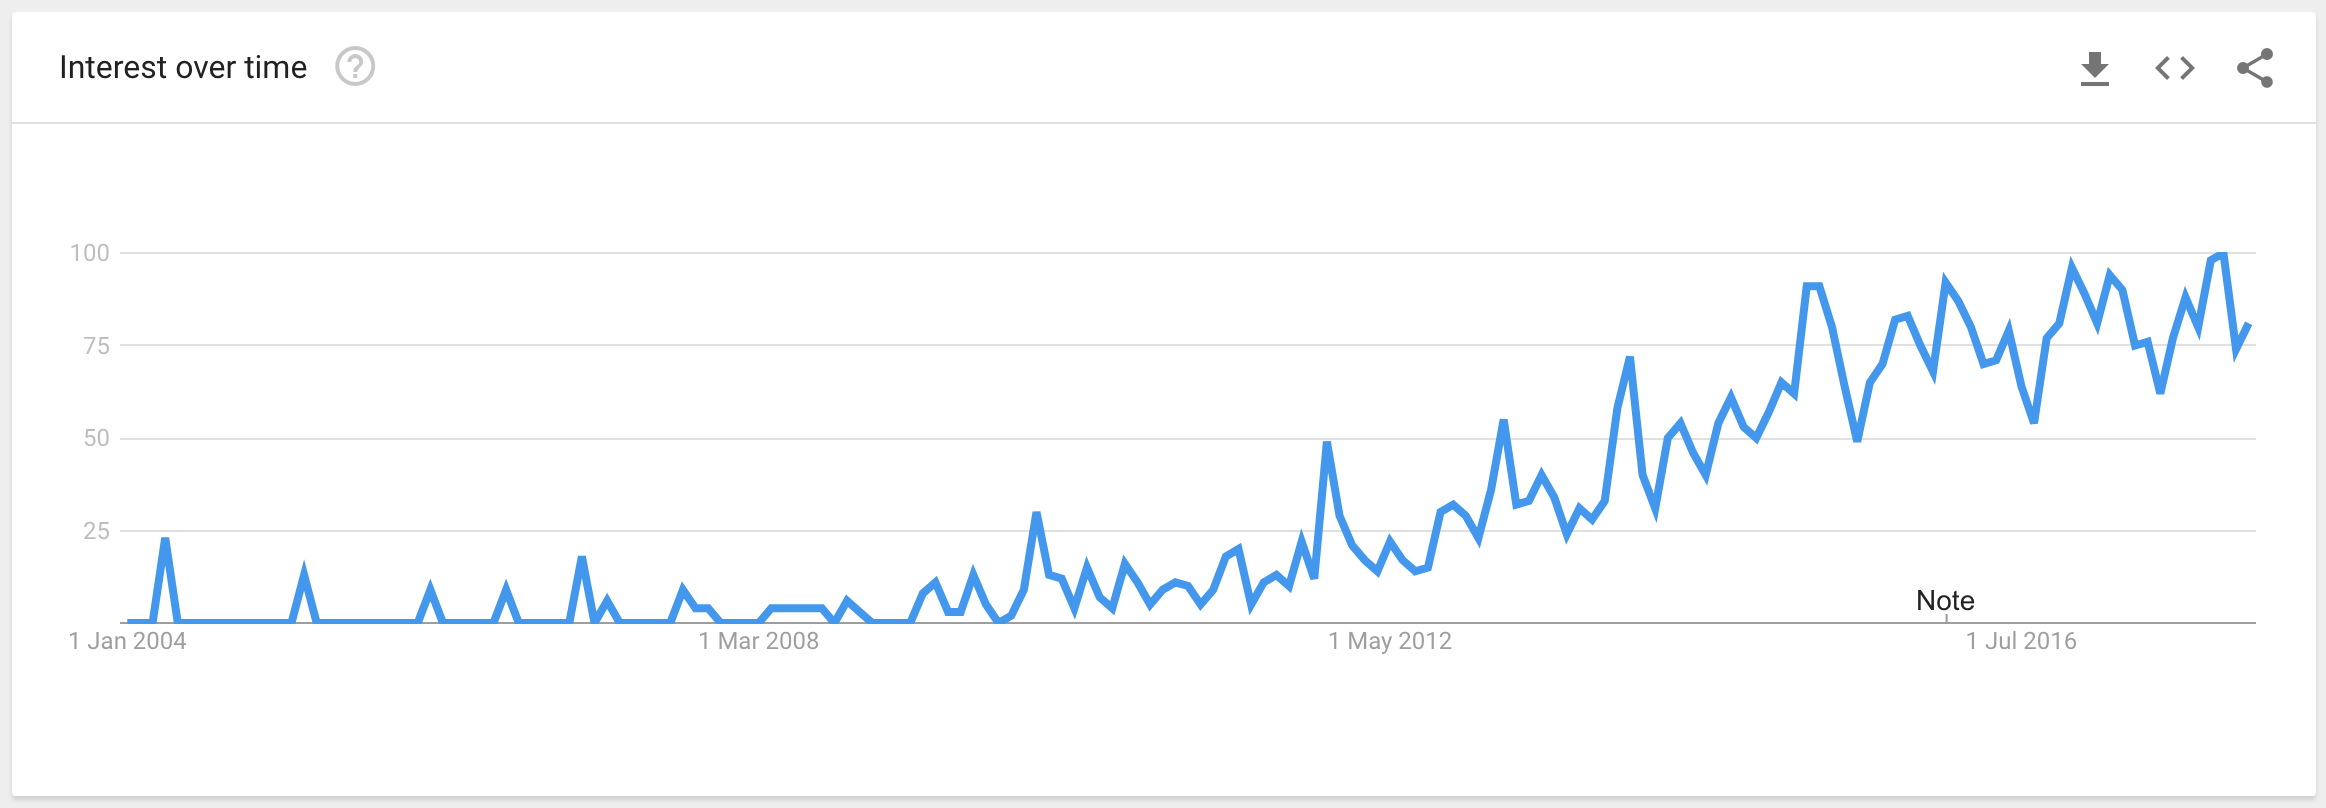
\includegraphics[width=\linewidth]{img/drone_interest_over_time_google.png}
  \caption{Google Trends for ``Drone Technology''. \cite{Google2018}}
  \label{fig:starship_citizen}
\end{figure}

Due to numerous advances in technology, drones are quickly advancing to the point where human input is no longer a necessity. This has led to many companies showing interest in integrating drones with their work in the coming years. \\

Although it may be an engineer's dream for a fully automated world, drones in particular are a harrowing reminder that there are real risks associated with them. There are already several incidents of drones crashing into planes and flying into areas they shouldn't, most notably near Heathrow airport\cite{BBCNews2017}. All of this provides motivation to introduce some form of autonomous air traffic control system to navigate these drones to their respective destinations in a safe manner.\\

However, prior work has been done on the routing and navigation aspect of such a system\cite{Balaji2017}. In order for drones to truly take over more aspects of our lives, we must look at how they can provide a tangible benefit to specific use-cases. There is no doubt that simply removing the human element can save costs drastically, and there is none more exciting an application than with physical delivery networks.

The main factors that could prompt higher adoption of drones for delivery networks are cost, delivery speeds, and convenience. As figure \ref{fig:drone_del_cost} shows, drones can be both faster and cheaper than existing deliver options that consumers have access to.
\begin{figure}[!hbpt]
  \center
  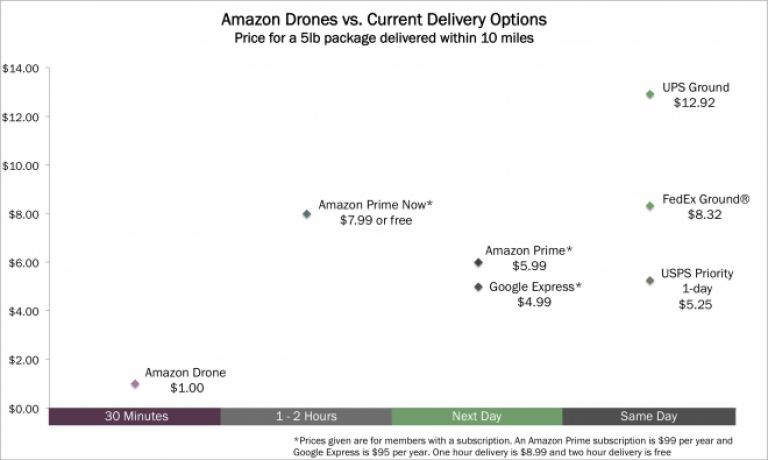
\includegraphics[width=\linewidth]{img/ark-invest-drones-analysis-768x460.png}
  \caption{How Amazon Air fits into the wider delivery market. \cite{Wang}}
  \label{fig:drone_del_cost}
\end{figure}

It appears then that Amazon stands to increase their margins considerably if they can successfully pull off their Prime Air initiative\cite{Welch2015}, but to do this they need to be able to handle the additional problems of scheduling and load balancing massive quantities of drones, on top of the existing routing problems. \\

In a more general sense, goods delivery networks have a lot to gain by optimising for profit, and to do this better we consider a variable delivery pricing mechanism that factors in the quality of service provided to the user. A high-priority product may warrant a higher delivery fee for quicker delivery but a similarly high penalty for being late. At the same time, a low-priority product may not have any such penalty, instead opting for a low delivery fee. Being able to factor this new fee model when scheduling tasks and allocating drones may be the next step in the ongoing automation of last-mile delivery\cite{Joerss2016}.

Regardless of how such a model is implemented, it needs to be tested thoroughly before being deployed into production with actual drones. Considering a typical delivery drone could cost around \$100 to \$500\cite{Menon2013}, and that there is likely be a lot of failure before a working implementation, there could be several hundreds of thousand dollars worth of losses. \\

Therefore, our best port of call is to simulate scenarios that are as close to the real world as possible. One tech firm investigating how to produce richer, meaningful and more realistic simulations is \textit{Improbable}\cite{ImprobableWorldsLtd.2018a} - a London-based tech startup actively developing a distributed simulation platform called \textit{SpatialOS}\cite{ImprobableWorldsLtd.2018b}. \\

We aim to leverage the power of SpatialOS to produce novel simulations of a drone delivery network. The simulation will build upon existing routing solutions\cite{Balaji2017} and would aim to schedule deliveries based on a Quality of Service value curve. Furthermore, we wish to show how the profitability of a drone delivery network with this form of scheduling might compare to delivery networks that utilise a different scheduling mechanism.

%**********************************************%
\newpage
\section{Background}
We first provide an insight into new developments in the physical delivery network sector, and then specifically considerations to account for when integrating drone technology in our day to day lives. Additionally we summarise prior work completed by Imperial students on an autonomous air traffic control system for drones. \\

We then continue to discuss methods of prioritising a delivery network for financial gain. Finally, we give details about Improbable's SpatialOS and the reasoning for using this platform for the drone simulation.

\subsection{Future of Delivery Networks}
From the ancient days of Assyrian trade in 19 BCE \cite{stearns2001the}, to the modern day online market - the ability to trade goods and services has had a profound impact on the way we live our lives. Thanks to globalisation and the explosion of the internet, we are now able to use a service such as Amazon Prime and get goods delivered within days, if not hours, of purchasing through a simple click. Through it all, physical delivery networks enable this online retail behemoth. \\

As technology evolves, so too will these delivery networks - and many companies are currently looking into how to leverage upcoming tech\cite{Lee2016} in order to generate hype for their business and, more importantly, increase their profit margins. Some promising developments are delivery robots, autonomous cars and, of course, drones.

\subsubsection{Delivery Robots}
Delivery robots are unmanned devices that are designed to be operated on pavements and cycle lanes at low speeds of about 4 miles per hour\cite{Lee2016}. Although the unmanned device market is in its infancy, there are already prototypes hitting the market such as Starship's robot\cite{Laris2016}, which can hold upto 20-25 pounds, and Dispatch's ``Carry''\cite{Kokalitcheva2016}, that holds up to 100 pounds.

\begin{figure}[!hbpt]
  \center
  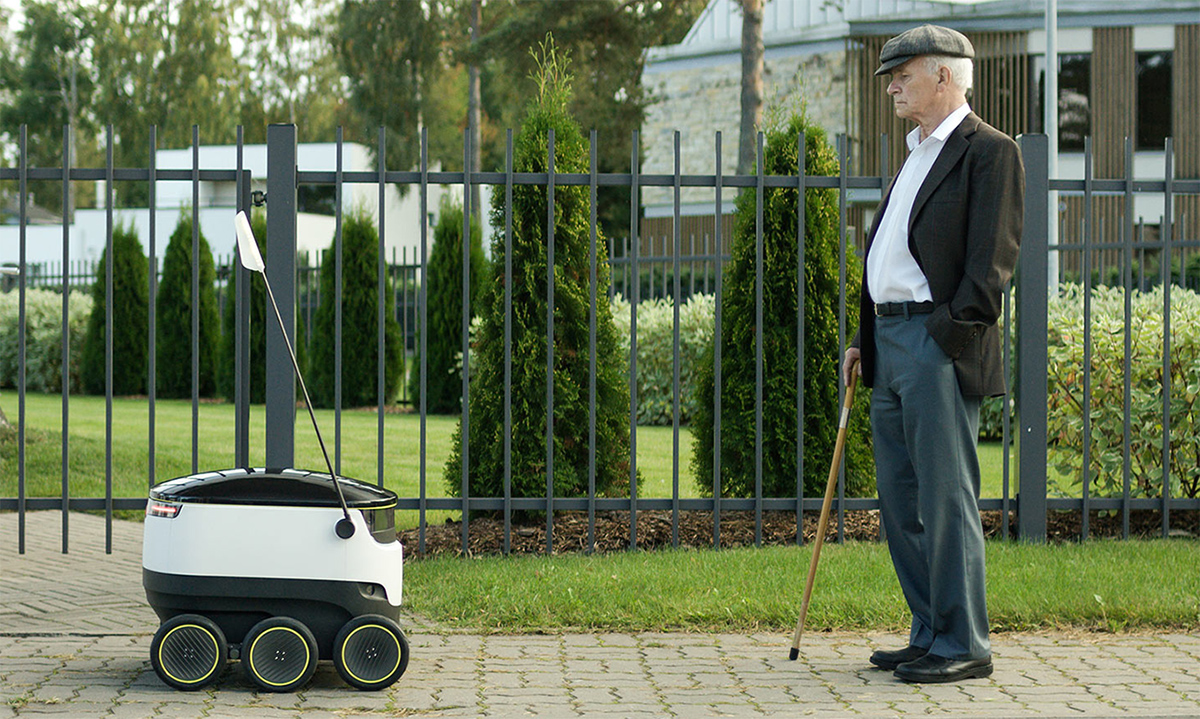
\includegraphics[width=\linewidth]{img/starship.jpg}
  \caption{Starship's robot confronting a senior citizen. Image from Engadget\cite{Souppouris2015}.}
  \label{fig:starship_citizen}
\end{figure}

Due to their on-the-ground nature, delivery robots are primarily designed for low-footfall suburban neighbourhoods, closed residential areas or campuses. They would be scheduled through an Uber-like application that may allow users to track the location of the robot, for the customer's knowledge, and to also unlock the robot once it reaches its destination\cite{Hohenadel2015}. \\

Thanks to their similarities to autonomous cars, they may have regulatory advantages compared to drones because much of the legislation coming through for autonomous vehicles can apply to delivery robots as well. However, there are profitability concerns because each robot can cost hundres of dollars and there is at this stage there is a high risk of failure, damage and even theft. \\

Despite some drawbacks, it is evident these robots are designed for short journeys in the so-called "first-mile delivery" sector - with exciting use cases being the delivery of flowers, groceries and possibly medication.

\subsubsection{Autonomous Vehicles}
Once the de-facto icon of science fictional futurism, autonomous cars are now a close reality. Companies such as Tesla are doing pioneering work in bringing self-driving cars\cite{Tesla2018} to the general consumer. Meanwhile, other businesses like Uber are experimenting with autonmous taxi services\cite{Gibbs2017}. \\

In fact, Google has obtained a patent for an autonomous delivery truck \cite{Hall-Geisler} with different compartments that could be unlocked by validated package recipients - much akin to an Amazon Locker-on-wheels. If not this, these vehicles could be used as an autonomous courier to pick-up locations that users could visit to retrieve their packages.

\begin{figure}[!hbpt]
  \center
  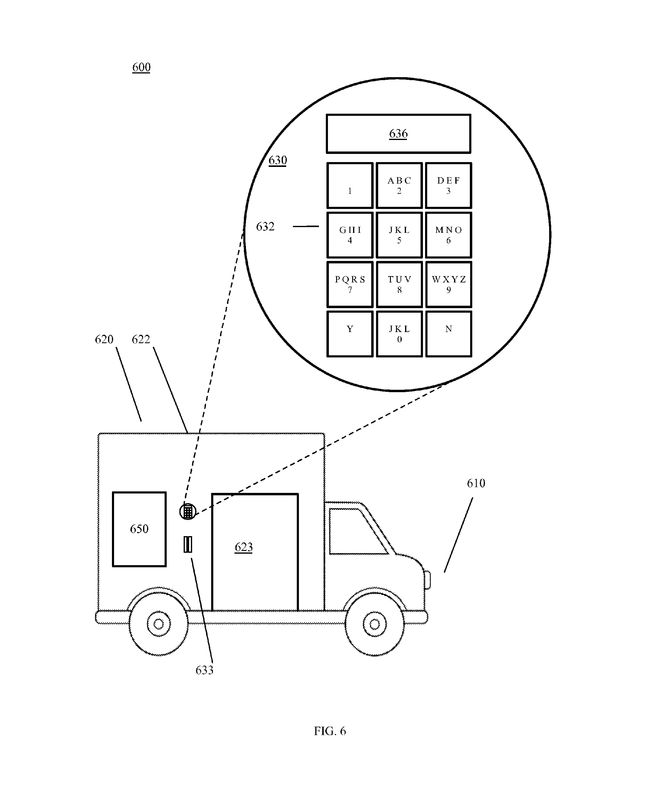
\includegraphics[width=0.4\linewidth]{img/google_truck_patent.jpeg}
  \caption{Illustration of Google's Delivery Truck. \cite{google_truck_patent}}
  \label{fig:google_truck_patent}
\end{figure}

Although current regulations dictate that a driver must remain present in the vehicle in the event of software performing differently to expections, this is a necessary precaution whilst driverless systems are still being tested - with further amendments to these laws in sight once these systems can be deemed safe for public use\cite{Bowcott2017}.

\subsubsection{Drones}
The concept of drones has been around for decades, particularly in the military, but only in recent times has the technology evolved to a point where anyone can walk into a consumer electronics store and purchase a drone for their own private use. Though these are manned, it is admirable that many witness the benefits of drones in film/television\cite{Verrier2015}, agriculture\cite{Jarman2016}, policing\cite{BBCNews2017a} and other exotic activities\cite{Roberts2016}. \\

Being able to fly allows drones to not be held hostage to traffic jams or congestion - after all, the sky is a far greater expanse than even the most intricate of road networks. Not only that, they can literally travel ``as the crow flies'' - allowing them to access remote and previously hard-to-reach areas.\\

Despite several near-misses \cite{Davies2017} and accidents\cite{BBCNews2016} at just Heathrow airpot alone, engineering teams across the world are working on ways to improve drone visibility to its surroundings - one such technology being automatic dependent surveillance-broadcast (ADS-B) \cite{Dillow2015}. Drones with ADS-B work by determining their own geolocation and velocity in order to broadcast this back to the global network.\\

ADS-B is already widely used in aircraft, enabling flight-tracking services such as flightradar24 to exist\cite{Flightradar242018}, but recent developments have allowed the ADS-B units to be compact and cost-effective enough to be suitable for drones. As more drones adopt this technology, instead of having to get instant updates from a drone directly, autonomous drone traffic control systems could make use of the shared global network for their scheduling and routing calculations. \\

Over time, an increasing percentage of the world's drones will likely join these shared autonomous systems. This could enable different delivery networks to manage their own fleets as their own air traffic controllers, all the while making use of the shared pool of readable data to identify, intercept and avoid drone collisions at the earliest stage in their pathfinding as possible.

\subsection{Amazon Prime}
Amazon Prime is a paid subscription service that Amazon offers to users, giving unlimited access to their video and music streaming services as well as providing free same-day and next-day delivery on a large majority of goods sold on their platform. The Prime service applies to products that are either sold directly by Amazon or fulfilled on behalf of a third-party merchant.

\subsubsection{Fulfilment by Amazon}
One of the services Amazon provides to merchants is the \textit{Fulfilment by Amazon} service, where goods are held at Amazon depots until a user purchases a product. The fee paid by the merchant for Amazon to take care of delivery depends on the duration of time the product is held by Amazon as well as the type of package and weight of the product.

\begin{figure}[!hbpt]
  \center
  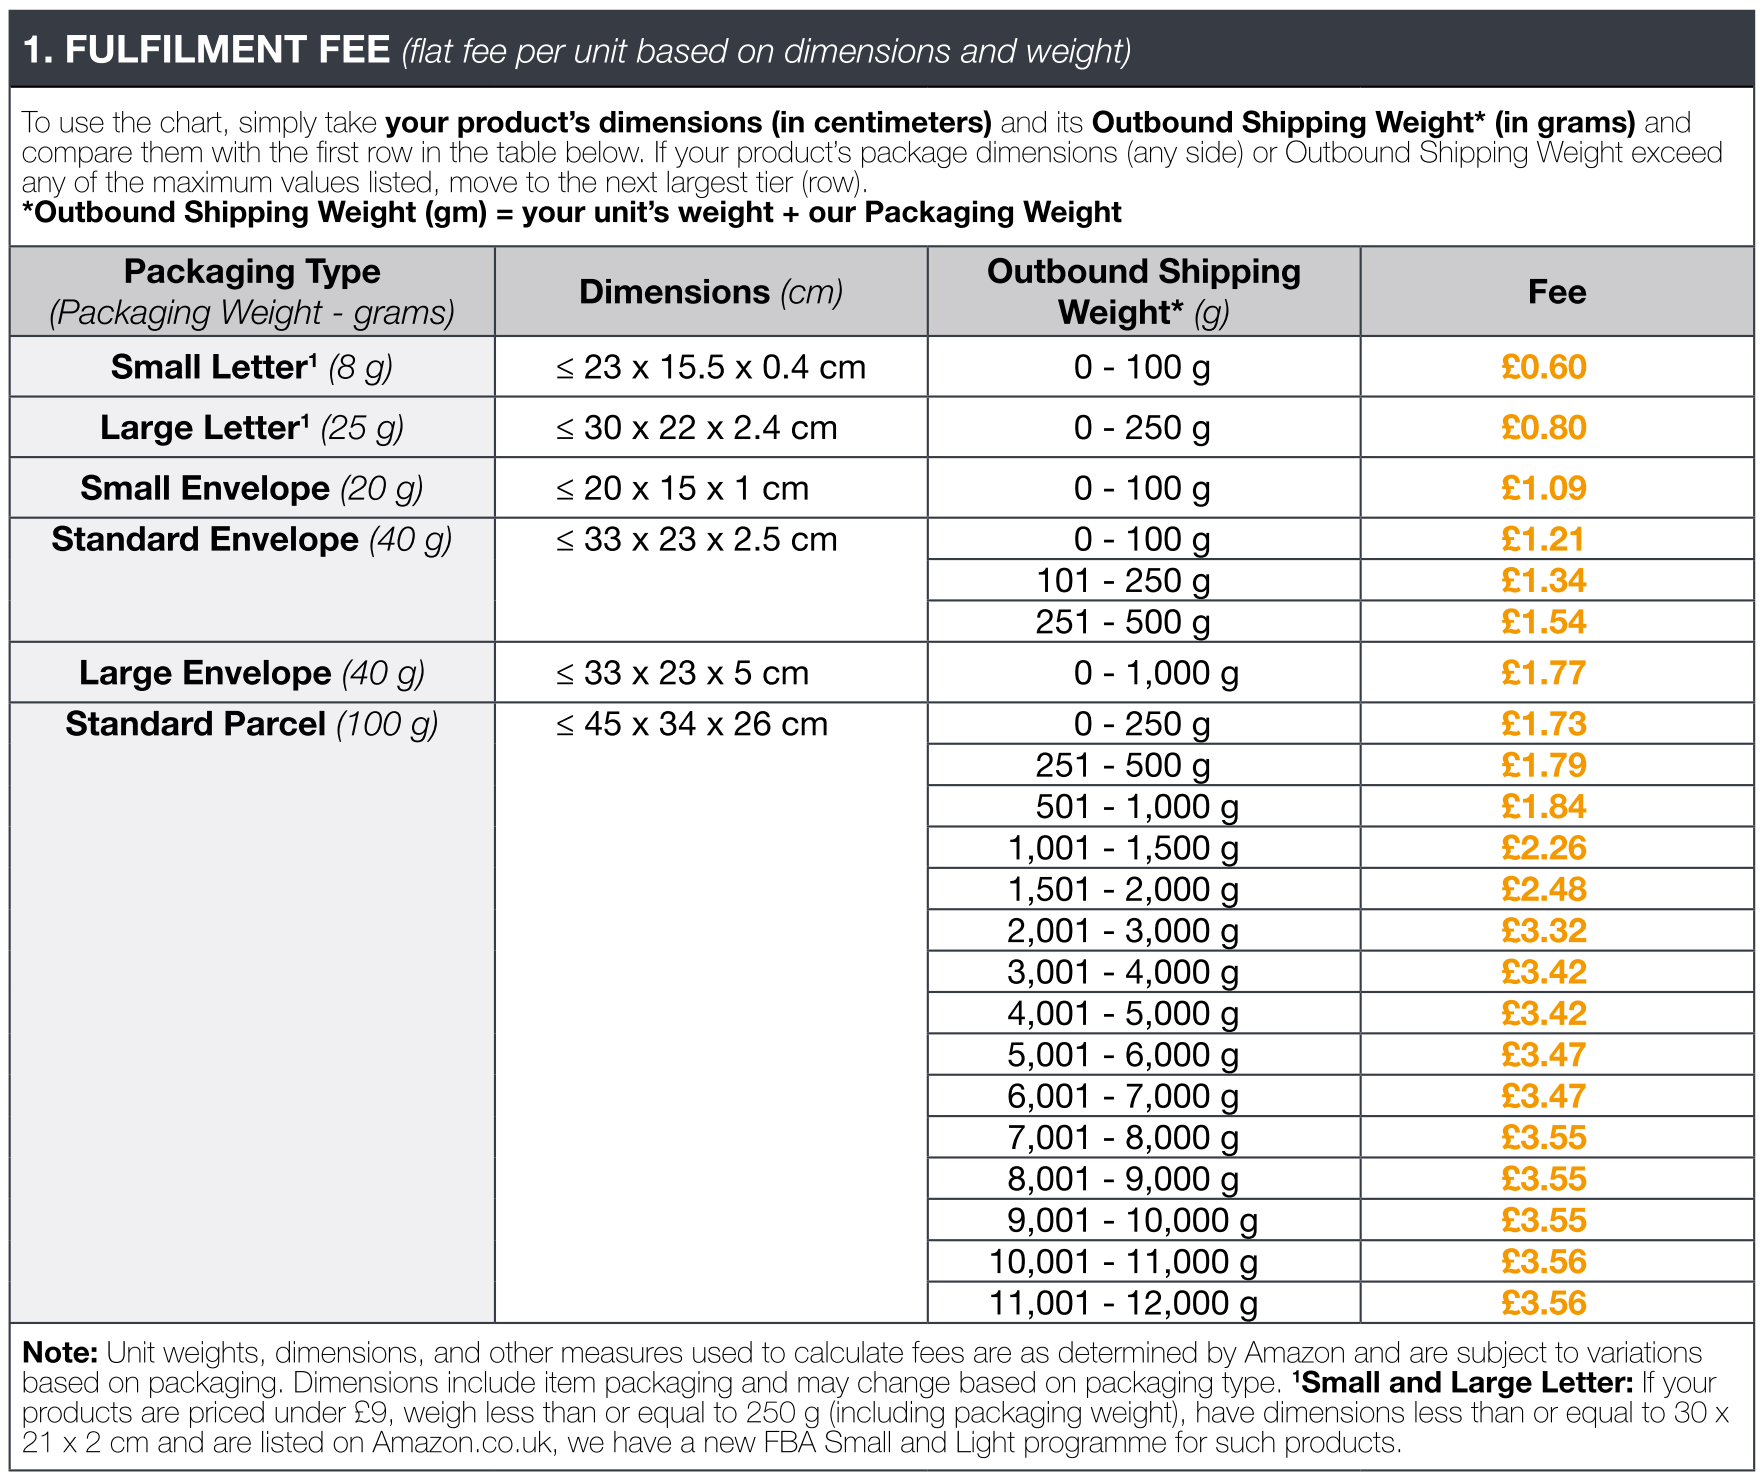
\includegraphics[width=0.9\linewidth]{img/fulfilled_by_amazon_table.png}
  \caption{Fulfilment fees for standard-size items on Amazon UK. \cite{Channel2017}}
  \label{fig:fulfilled_by_amazon_table}
\end{figure}

An incentive for merchants to join this scheme is to attract customers with the same-day and next-day delivery that Amazon Prime offers. This allows them to piggy-back off the existing delivery network that Amazon has developed for significantly lower fees (Figure \ref{fig:fulfilled_by_amazon_table}) than if they were to store the package and source a distributor for themselves.

\subsubsection{Amazon Prime Air}
In December of 2013, Amazon announced their intentions to research and develop their own drone delivery service dubbed \textit{Amazon Prime Air} \cite{Amazon.comInc.2013}. Amazon intends this service to deliver packages within 30 minutes of an order being placed, with a maximum package weight of 5 pounds (approximately 2.27 kg).\\

Following this, in November of 2015 the company enlisted the help of Jeremy Clarkson to give a closer look at a more developed drone prototype \cite{Amazon.comInc.2015b}, describing how Prime Air would fit into the lives of modern families. Just over a year later, Amazon released a video demonstrating a fully autonomous delivery using Prime Air \cite{Amazon.comInc.2016}.

\begin{figure}[!hbpt]
  \centering
  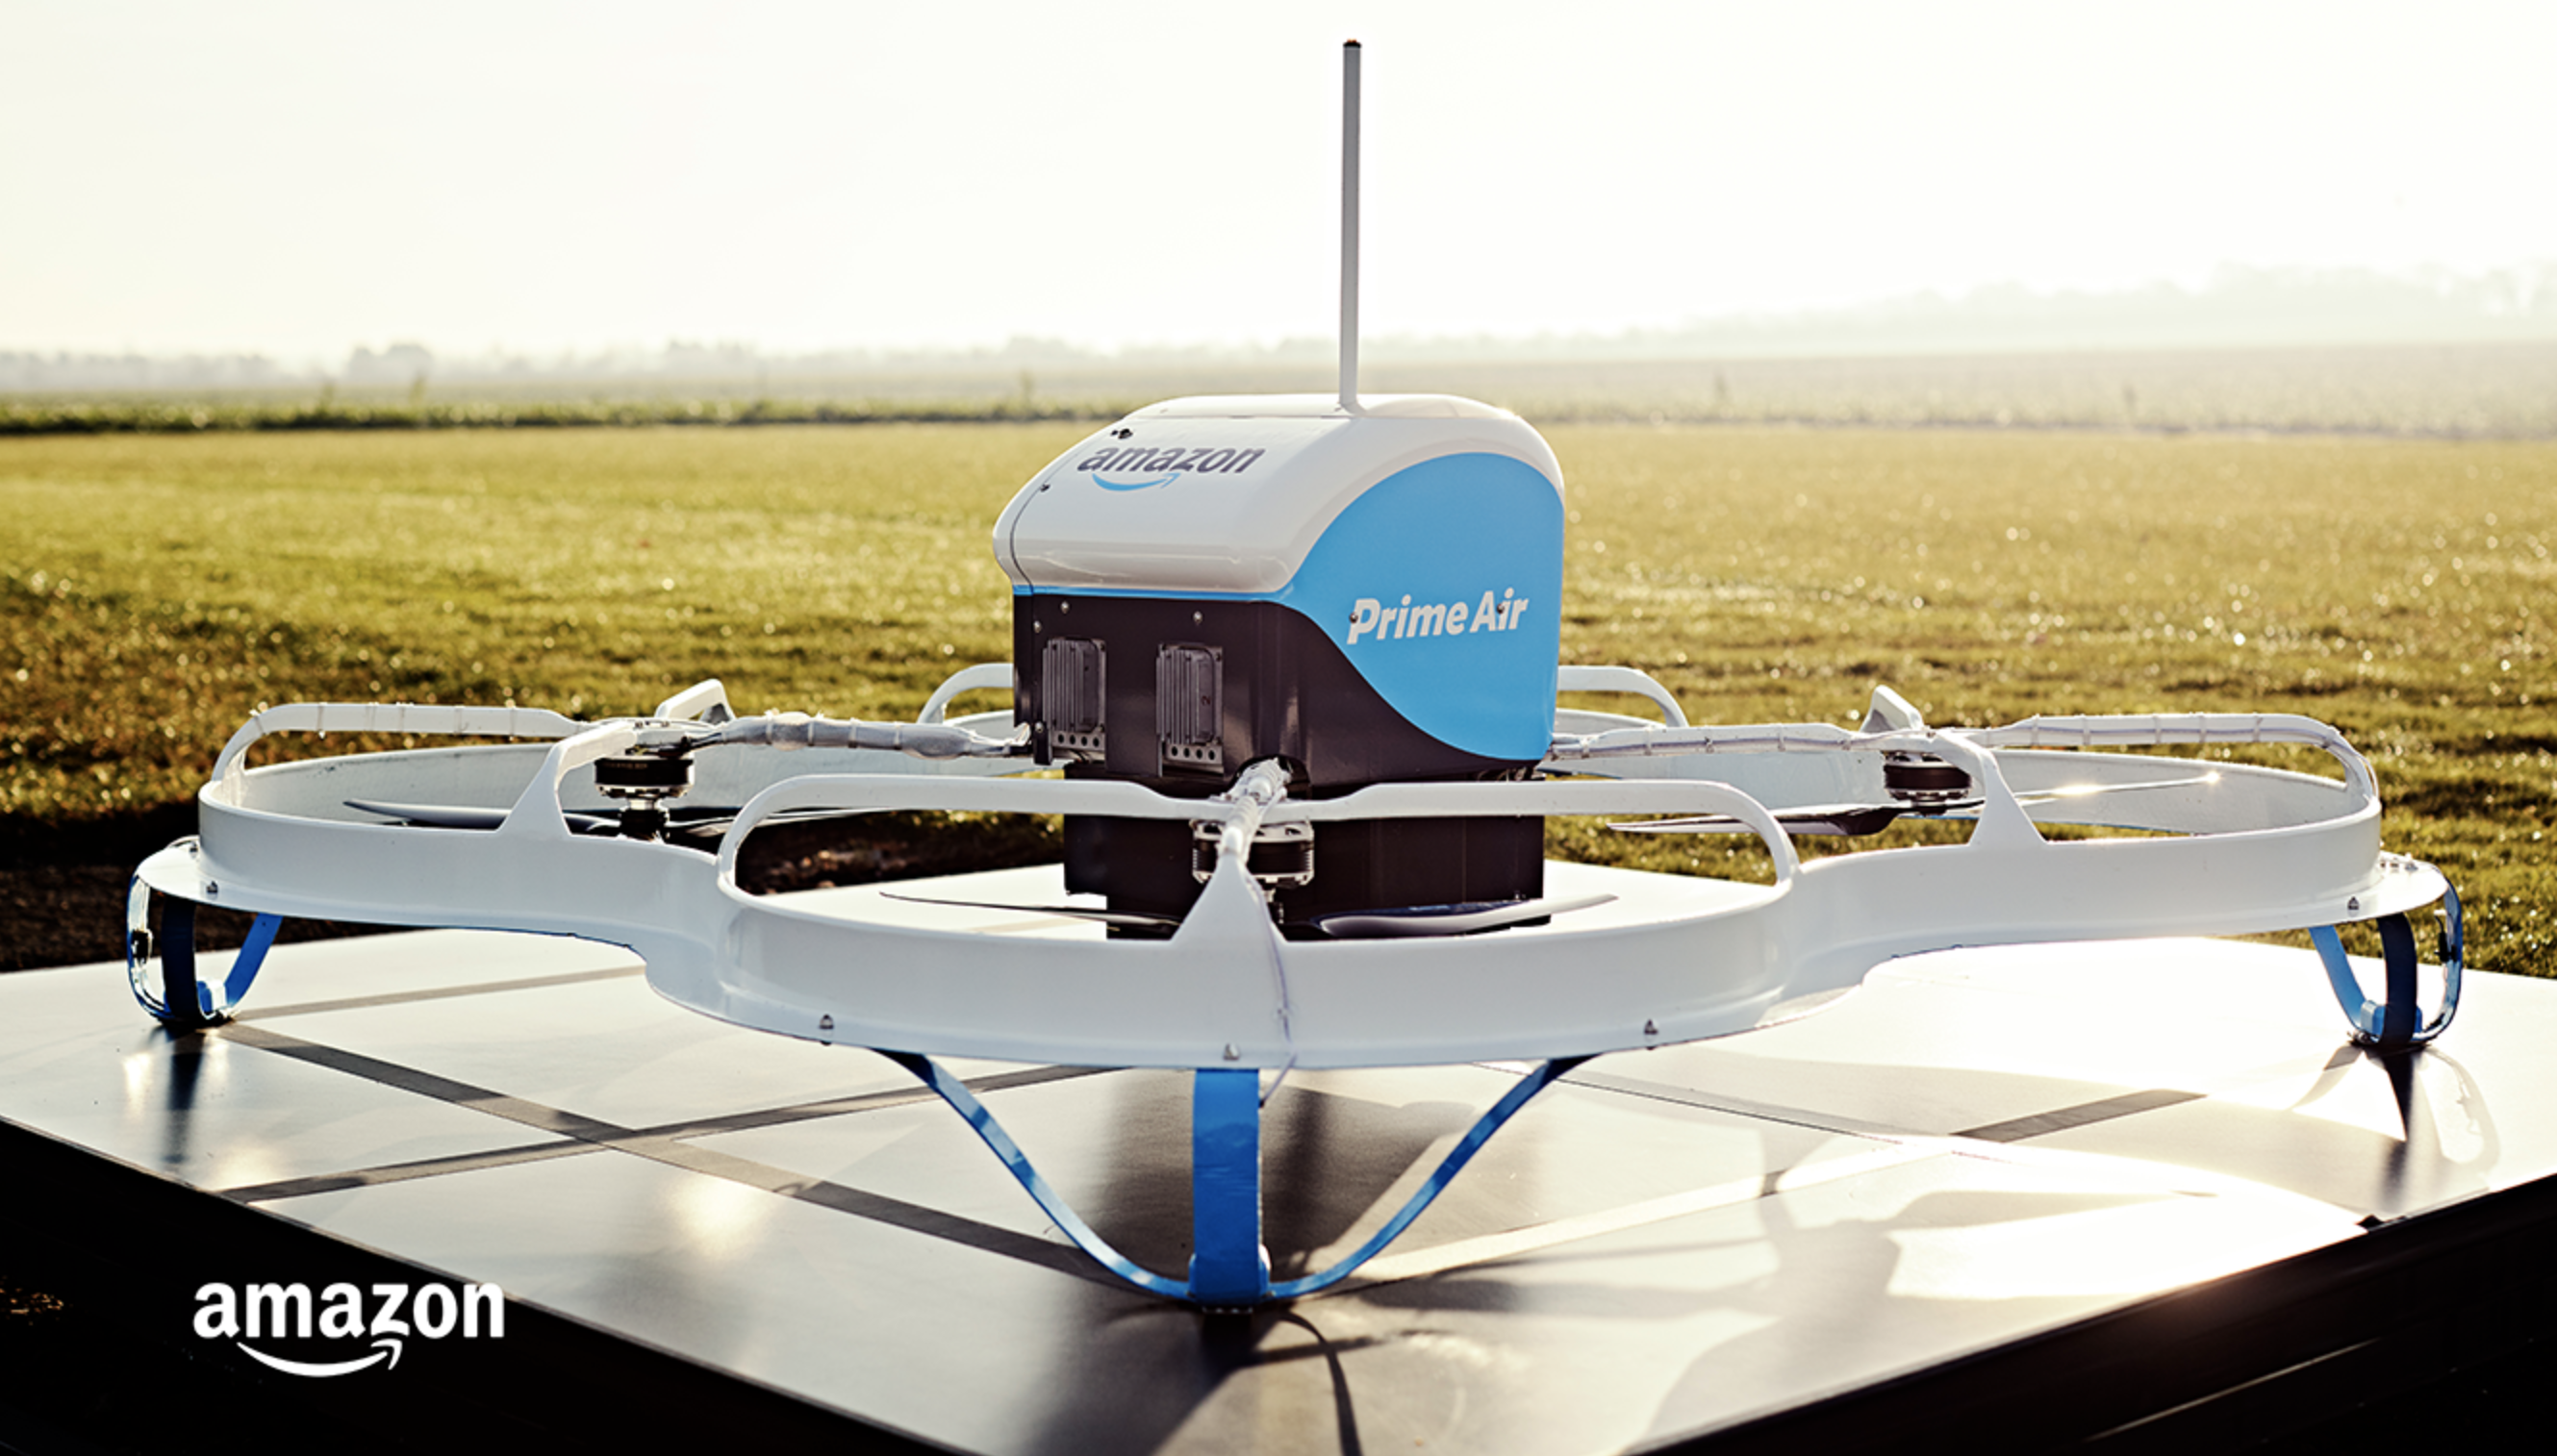
\includegraphics[width=0.6\textwidth]{img/amazon_prime_air_drone.png}
  \caption{One of Amazon's Prime Air prototypes. \cite{Amazon.comInc.}}
  \label{fig:prime_air_example}
\end{figure}

One of the many roadblocks to scale this technology out across the country is regulatory approval. Since drones are a new technology that improve in leaps and bounds each year, authorities and enterprises are careful to make hasty judgements that either hamper drone adoption or cause civilian harm. To this end, Amazon are also suggesting proposals to how airspace can be best utilised by drones. \cite{Amazon.comInc.2015} \cite{Amazon.comInc.2015a}

\subsection{Drone Considerations}
Drones stand to be a revolutionary part of our lives as we welcome the new, incoming era of automation. However, to be practical there are a few key concepts one must understand to ensure that they remain a help and not a hinderence to mankind.

\subsubsection{No Fly Zones}
No Fly Zones (which we will abbreviate as NFZs) are geographical areas where a drone is not allowed to enter or fly at any altitude. Examples of these may include Hyde Park, Buckingham Palace, airports and military locations. Typically these are static obstacles that will always remain a NFZ, however we could also consider cases when they could be created dynamically.\\

Suppose there was an issue of national security, it would be beneficial for the security and intelligence services to set up a temporary NFZ around areas where they deem a risk so that they can conduct their own operations without worry of external parties interfering with the situation.

\subsubsection{Other Drones}
Naturally we would want to make sure that we avoid colliding into other drones as well. In a perfect system, a single air traffic controller would have totalitarian dominance over all drones that take to the skies - however this is not \textit{Black Mirror} and we have to assume that there will always be drones that this system will not be able to control or predict. \\

Nonetheless, a system can ensure that it navigates drones under its control as best as it can, avoiding these external drones and other rogue drones that may be flying with the sole intention of causing problems to others.

\subsubsection{Manned Aviation}
Manned Aviation is any form of airborne transport with humans on board. This would include passenger jets, private jets, helicopters and other miscallaneous vechicles. For simulation purposes, we can consider these to have straight paths from a start to an end because relative to the zig-zagging of drones - they are effectively straight. \\

It is paramount to avoid collisions with manned aviation because there is a high risk of human calamity, in addition to the bad press and financial costs associated with such an air traffic incident.

\subsubsection{Toll Zones}
Toll Zones are geographical areas where a drone has to pay an extra fee to pass through at any altitude. It is a very similar idea to the one that led to Congestion Charges being applied to much of central London. By restricting certain areas only to those who are willing to pay the fee to use the airspace, it reduces the density of air traffic in a specific area. These charges could also be used as an incentive to reduce pollution in the toll zone, and the additional revenue generated by the toll fees could be used towards the drone-related systems in place within the zone.

\subsection{Autonomous Air Traffic Control (AATC)}
\subsubsection{What is AATC?}
During the Autumn Term of the 2016-17 academic year, several students undertook a group project in association with Microsoft and Altitude Angel to produce an autonomous air traffic control system. The goal of the project was to safely navigate drones from their start to their end goals, whilst avoiding obstacles and taking the shortest possible path to minimise battery use.

\subsubsection{Technical Overview}
AATC has a simple client-server architecture, where drones connect to the REST service to send their telemetry information and goal waypoints every second. The server sends back direction recommendations to navigate the drone to its destination. \\

Because it would have been too expensive to trial the system on actual drones, a test bench was also implemented that would simulate the drones polling the server and responding to its recommendations. This test bench produced a set of simulation data, that is then available to view on the AATC visualiser. \cite{Balaji2017a}

\begin{figure}[!hbpt]
  \center
  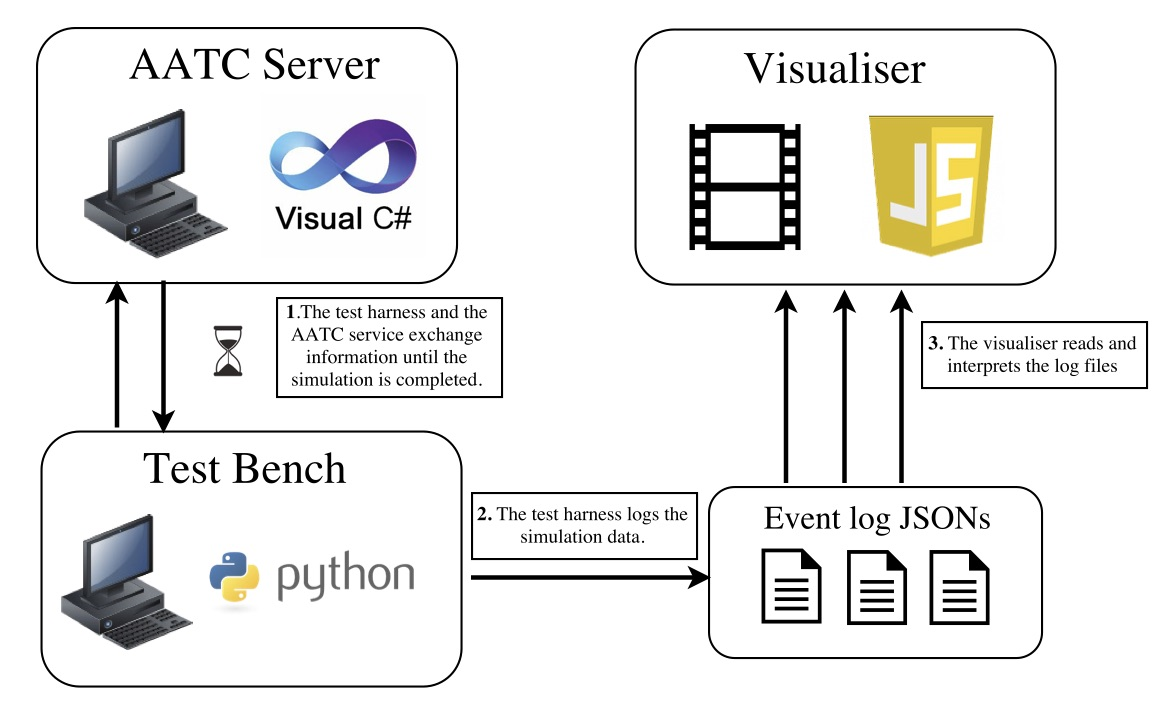
\includegraphics[width=\linewidth]{img/aatc_tech_overview.jpg}
  \caption{Technical Overview of AATC. \cite{Balaji2017}}
  \label{fig:aatc_tech_overview}
\end{figure}

The system was designed with three challenges in mind. The first challenge was to route drones from their origins to their destinations, and secondly, to ensure they avoided collisions with both static and dynamic obstacles - such as the ones mentioned in Section 2.1. The last challenge is to design the system in such a way that it would be able to scale to hundreds and thousands of drones. \\

\newpage
To this end, a \textit{Global Layer} was built to deal with static obstacles (such as NFZs) by calculating a path for the drone around NFZs before it begins its journey. The second problem was tackled with a \textit{Reactive Layer} that handles non-static obstacles (such as manned aviation and other drones). This is the layer that would be providing the real-time updates to drones as they poll the server every second. \\

\begin{figure}[!hbpt]
  \center
  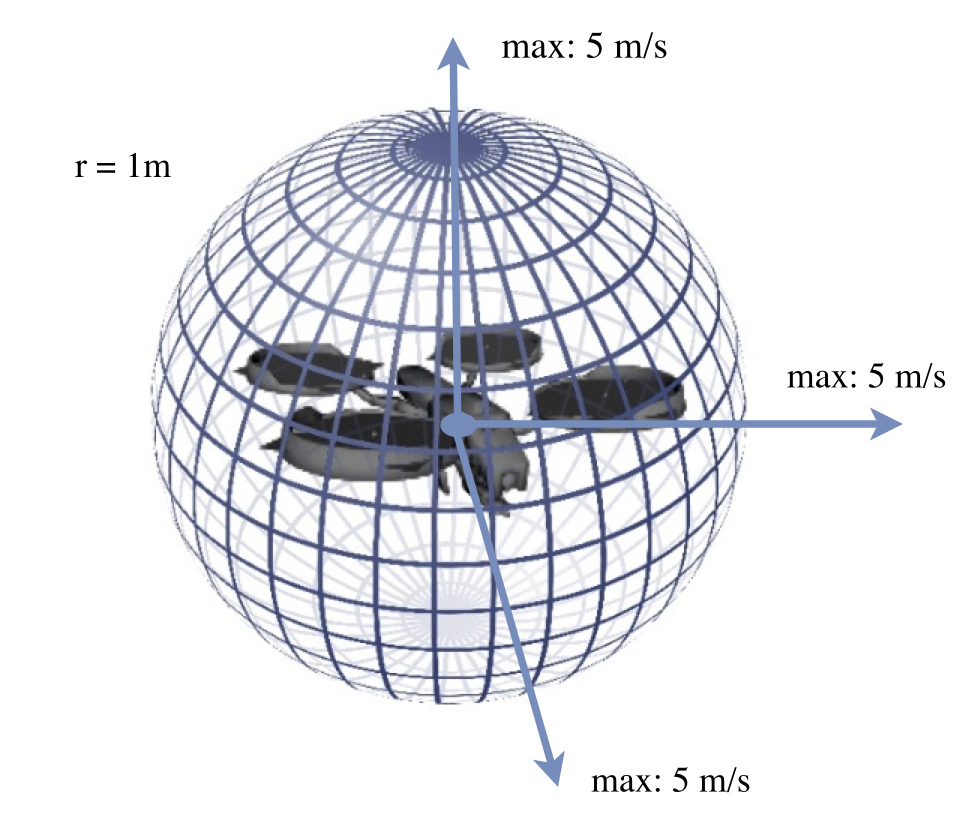
\includegraphics[width=0.8\linewidth]{img/edrone.jpg}
  \caption{The default AATC drone model. \cite{Balaji2017}}
  \label{fig:edrone}
\end{figure}

Only one drone type was used in AATC, with its specification outlined above in Figure \ref{fig:edrone}. It has a radius of 1m and a maximum velocity in any direction of 5 metres per second.

\subsection{The Global Layer}
The Global Layer holds the static representation of the world so that given a start and end, it can compute an optimal set of waypoints that a drone should follow - thereby dealing with AATC's path-finding problem.

\subsubsection{Dijkstra's Algorithm}
Dijkstra's algorithm is a popular algorithm to find the shortest paths between nodes in a graph. When using a co-ordinate grid system, each coordinate could represent a node in a graph and thus the algorithm can also be used to find the shortest path between a source and destination. \\

However, in the real world, we also have to consider the cost of computation and potentially make use of heuristics in order to return the shortest path given a limited amount of time. Especially in the drone case, we want to compute a good path as quick as possible in order to let the drone proceed along its way.

\subsubsection{A* Algorithm}
Enter, the A* algorithm. This algorithm is a generalisation of Dijkstra's algorithm that reduces the number of nodes explored during the search process by use of a heuristic - typically a minimum distance to the destination. A benefit over Dijkstra in particular is that it considers the distance already traveled into account, which aids the heuristic mechanism. \\

Naturally, by searching less nodes on a graph, less computation is performed and therefore A* has better performance than just using a pure form of Dijkstra's algorithm.

\begin{figure}[!hbpt]
  \center
  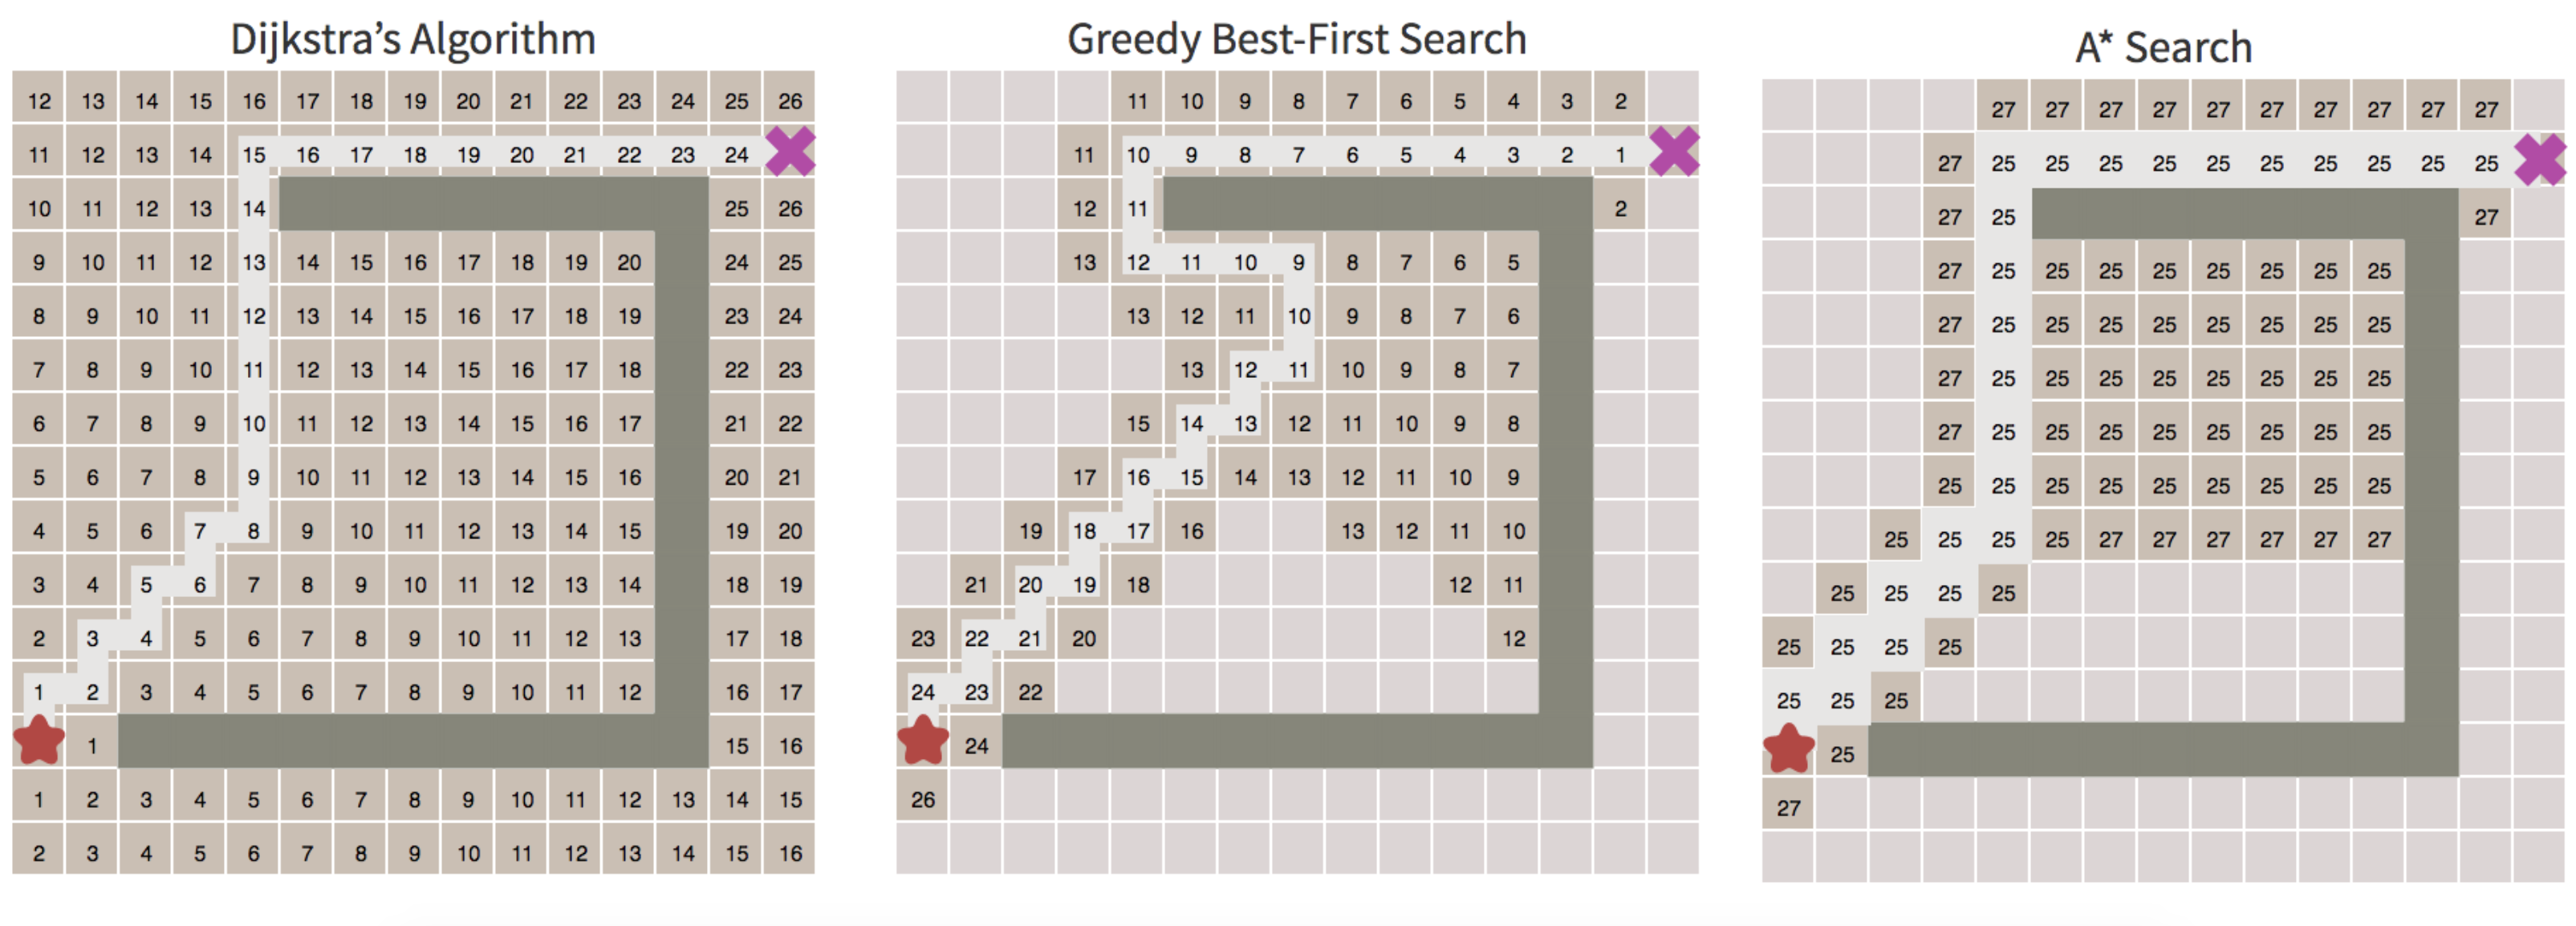
\includegraphics[width=\linewidth]{img/search_comparison.png}
  \caption{Comparing popular search algorithms. \cite{Balaji2017}}
  \label{fig:search_comparison}
\end{figure}

But for all these positive aspects, one must remember that our use for this algorithm is to compute paths in a real world, which is not necessarily split up into a nice, clean grid. So we turn our attention to a modification of the A* algorithm: Theta*.

\subsubsection{Theta* Algorithm}
The Theta* algorithm is an any-angle pathfinding algorithm based on the A* algorithm that introduces Line of Sight (LOS) checks, which means that each jump from node to node in the returned path can be at any angle and not just up, down, left or right. This neat addition allows Theta* to be capable of finding near-optimal paths with a runtime comparable to A* \cite{Uras2015}. \\

\begin{figure}[!hbpt]
  \center
  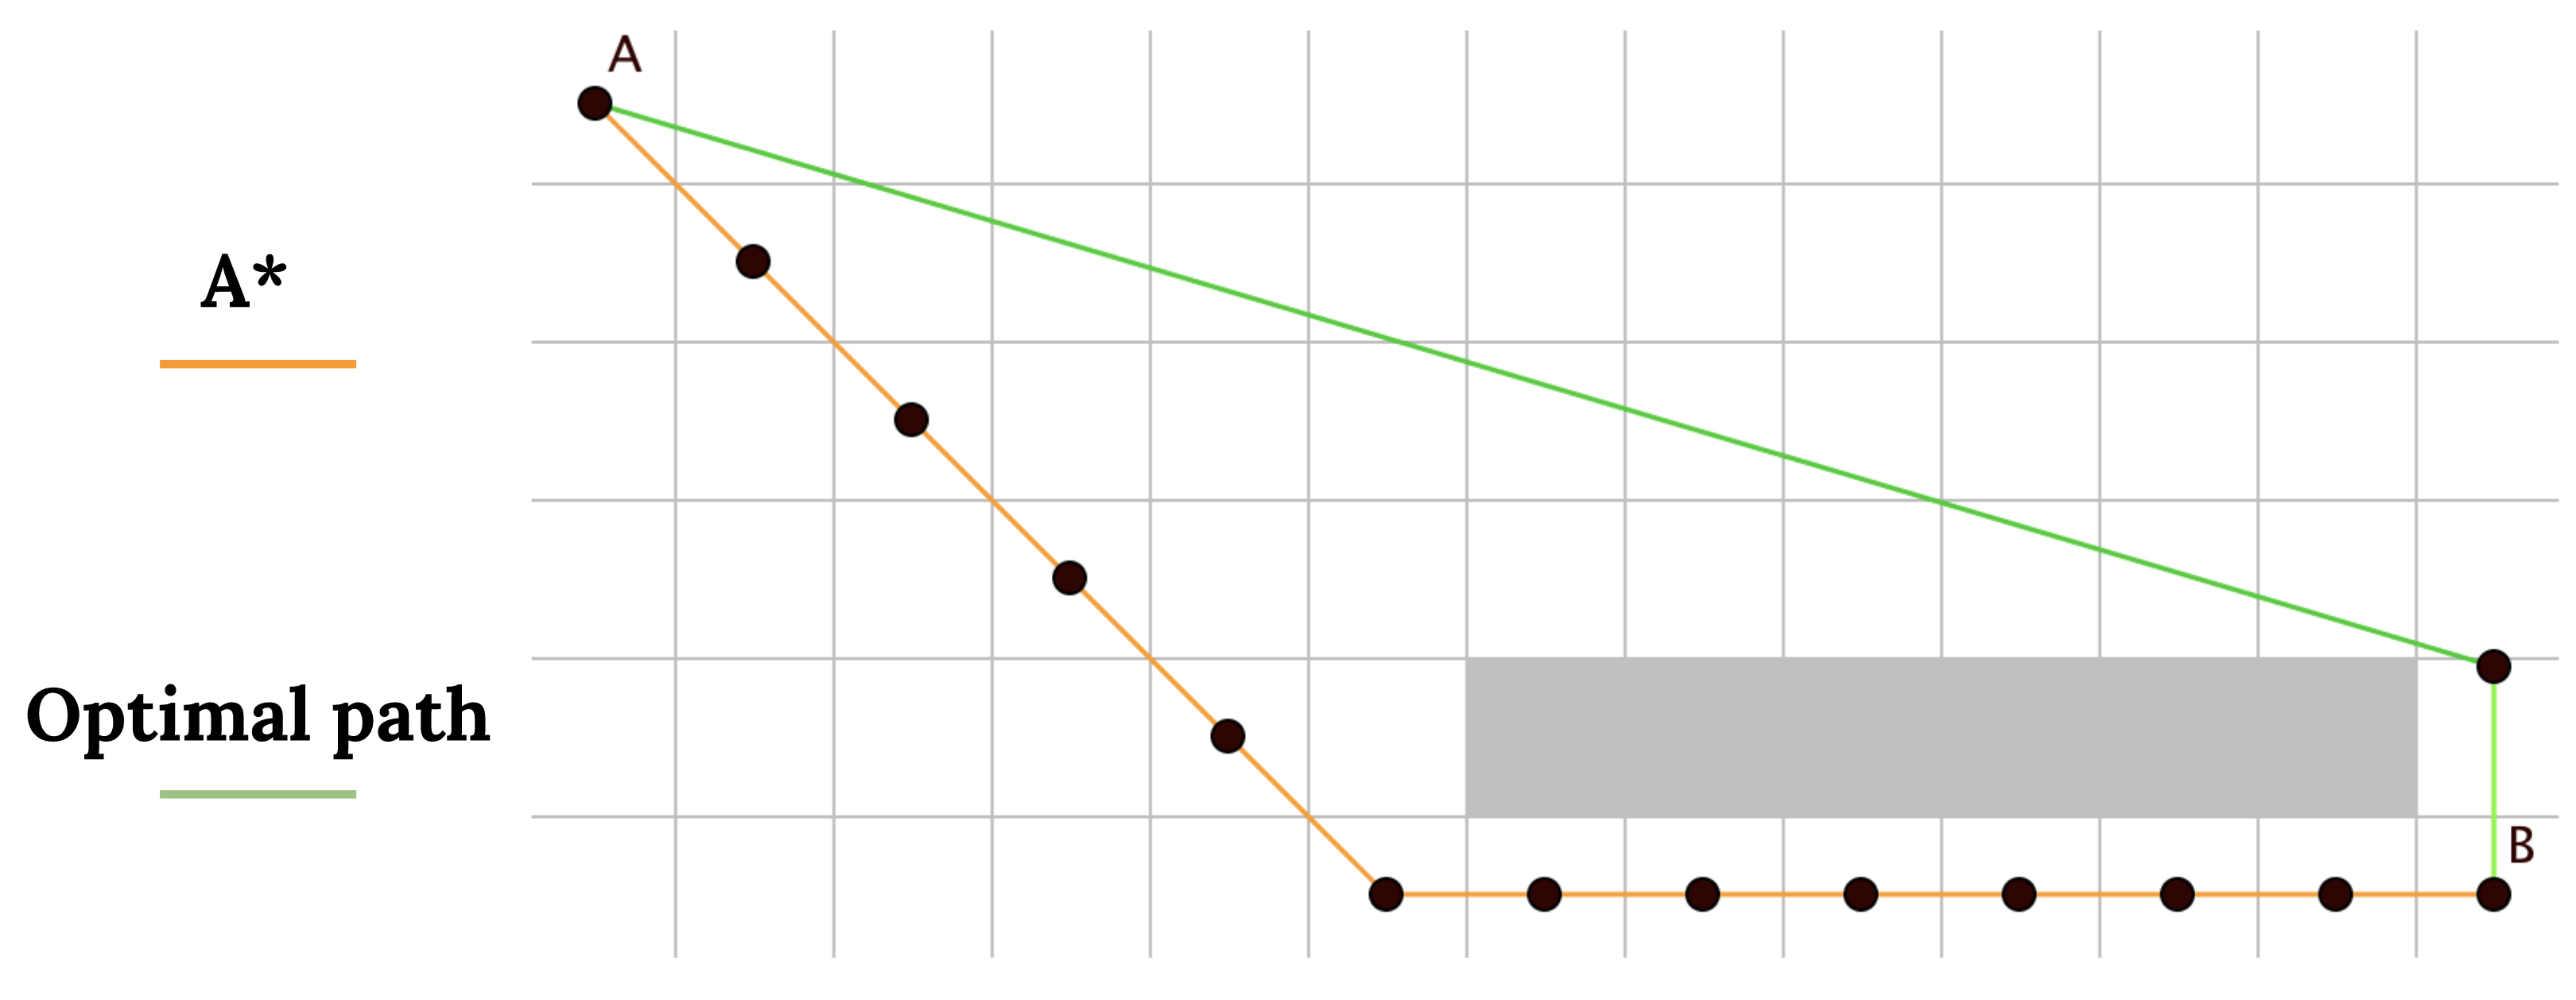
\includegraphics[width=\linewidth]{img/a_star_vs_optimal.png}
  \caption{A* vs Optimal Path. \cite{Balaji2017}}
  \label{fig:a_star_vs_optimal}
\end{figure}

Being able to get as short a path as possible is absolutely vital in the drone use-case because they have limited flying time. After all, their batteries can only last so long before they need to be recharged. Therefore, it is important to ensure drones travel as little distance as possible in order to maximise the number of times they can be used between charges.

\newpage
\subsubsection{Lazy Theta* Algorithm}
A further optimisation is to reduce the number of LOS checks performed, as found in another paper by the original authors of the Theta* algorithm\cite{Nash2010}. This algorithm assumes every node is in line of sight of its parent, and the LOS check is only performed once the child node is expanded on. If this turns out to be false, then the algorithm defaults to a typical A* approach. Reducing the number of LOS checks therefore improves the algorithm's overall performance.

\subsubsection{Conclusions}
As seen on Table \ref{tab:aatc_exec_time}, A* has far better execution times than both Theta* variants but when we get to Table \ref{tab:aatc_total_drone_distance} it is evident that Lazy/Theta* produces better paths because the total distance travelled by drones is fewer. Therefore, Lazy Theta* was chosen as the core algorithm for the Global Layer.

\begin{table}[!hbpt]
\centering
\begin{tabular}{|l|c|c|}
\hline
\multicolumn{1}{|c|}{Test Case} & A* & \multicolumn{1}{l|}{Theta* and Lazy Theta Star} \\ \hline
Queen Threat & 6.11 & 5.98 \\ \hline
The Imperial Tunnel & 10.83 & 10.22 \\ \hline
The Great London Beehive & 52.63 & 49.77 \\ \hline
The Nightmare of Hyde Park & 118.4 & 115.32 \\ \hline
The Great Wall of Imperial College & 16.37 & 15.46 \\ \hline
Multi Drone collision & 15.27 & 14.82 \\ \hline
\end{tabular}
\caption{Total path distances for all drones (in km). \cite{Balaji2017}}
\label{tab:aatc_total_drone_distance}
\end{table}

\begin{table}[!hbpt]
\centering
\begin{tabular}{|c|c|c|c|}
\hline
Test Case                          & A*                                                          & \multicolumn{1}{l|}{Theta*}                                   & \multicolumn{1}{l|}{Lazy Theta*}                              \\ \hline
Imperial Tunnel                    & \begin{tabular}[c]{@{}c@{}}118\\ 120\\ 121\end{tabular}     & \begin{tabular}[c]{@{}c@{}}141\\ 138\\ 137\end{tabular}       & \begin{tabular}[c]{@{}c@{}}124\\ 132\\ 129\end{tabular}       \\ \hline
Imperial Tunnel Mean               & 119.7                                                       & 138.7                                                         & 128.3                                                         \\ \hline
The Great London Beehive (GLB)           & \begin{tabular}[c]{@{}c@{}}859\\ 916\\ 894\end{tabular}     & \begin{tabular}[c]{@{}c@{}}1318\\ 1486\\ 1555\end{tabular}    & \begin{tabular}[c]{@{}c@{}}1166\\ 1075\\ 1201\end{tabular}    \\ \hline
The GLB Mean                       & 889.7                                                       & 1453                                                          & 1147.4                                                        \\ \hline
The Nightmare of Hyde Park (NHP)        & \begin{tabular}[c]{@{}c@{}}9771\\ 9687\\ 10118\end{tabular} & \begin{tabular}[c]{@{}c@{}}28436\\ 27970\\ 28273\end{tabular} & \begin{tabular}[c]{@{}c@{}}21330\\ 24786\\ 21609\end{tabular} \\ \hline
The NHP Mean                       & \multicolumn{1}{l|}{9858.7}                                 & \multicolumn{1}{l|}{28226.4}                                  & 22575                                                         \\ \hline
The Great Wall Of Imperial College (GWIC) & \begin{tabular}[c]{@{}c@{}}394\\ 447\\ 416\end{tabular}     & \begin{tabular}[c]{@{}c@{}}913\\ 910\\ 912\end{tabular}       & \begin{tabular}[c]{@{}c@{}}838\\ 840\\ 841\end{tabular}       \\ \hline
The GWIC Mean                      & 419                                                         & 911.7                                                         & 839.7                                                         \\ \hline
\end{tabular}
\caption{Execution times for pathfinding algorithms on AATC test cases. \cite{Balaji2017}}
\label{tab:aatc_exec_time}
\end{table}

\newpage
\subsection{The Reactive Layer}
Given the list of waypoints that the Global Layer generates, the Reactive Layer's task is to provide the right speed and direction to drones whilst taking into consideration any dynamic obstacles that the drone may face, such as manned aviation, other drones and potentially dynamic NFZs.

\subsubsection{Artificial Potential Fields (APF)}
A novel way to approach this layer is to create an Artificial Potential Field (APF) in the area the drone operates in, and give each point in this field a potential\cite{Zhu2016}. By having a low potential for the destination and large potentials at obstacles, the drone simply has to move in a way to get to point of lowest potential. It is analogous to a magnet in a magnetic field, repelled by obstacles and attracted to its destination. \\

Although one might argue that the Global Layer is not needed anymore because the Reactive Layer solves the pathfinding problem, there are a few issues that arise with this idea. As Figure \ref{fig:apf_comp} shows, a U-shaped object poses a problem because the drone may be attracted to the destination and then quickly repelled by the obstacle, and then back to being attracted - and this cycle is seemingly endless.

\begin{figure}[!hbpt]
  \center
  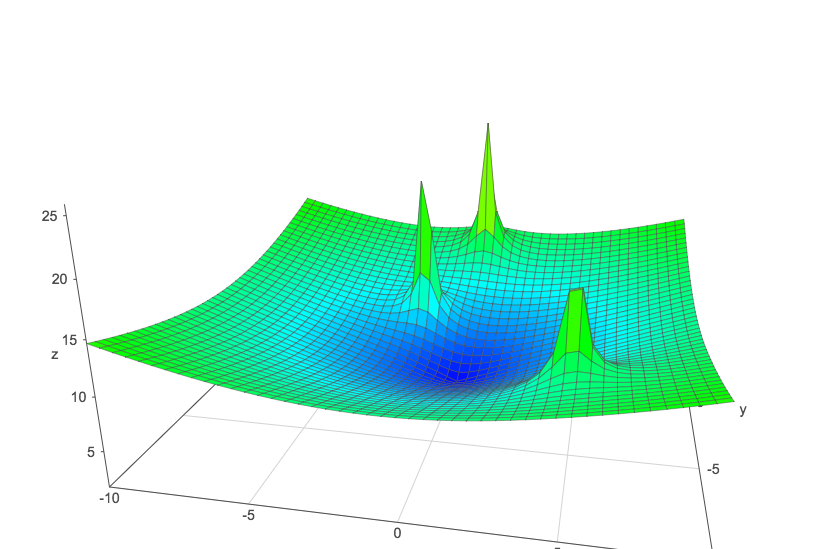
\includegraphics[width=0.9\linewidth]{img/obst.png}
  \caption{APF with obstacles (green peaks) and a destination (blue trough). \cite{Balaji2017}}
  \label{fig:obst}
\end{figure}

By introducing a random element, as in Rotating APF, the object is repelled in a slightly different direction each time to make it out of the trap and eventually reach its destination. Even this method, however, does not actually guarantee that the drone makes it past the U-shaped obstacle because it depends on how the random element behaves and also whether the drone has enough battery to be loitering for long.

\begin{figure}[!hbpt]
  \center
  \includegraphics[width=\linewidth]{img/apf_comp.png}
  \caption{Pure APF vs Rotating APF vs AATC Implementation. \cite{Balaji2017}}
  \label{fig:apf_comp}
\end{figure}

Clearly, integrating both layers proves most fruitful - as the waypoints generated by the Global Layer are used to quite literally navigate around the problematic aspects of the Reactive Layer. This integration that was implemented in the AATC project.

\subsubsection{Equations for APF}
The full set of equations used to obtain the recommended unnormalized velocity $v_{raw}$ of the drone is:
$$U_a = \rho_ad_{goal}$$
$$U_r =  \begin{cases}
      \rho_r\frac{1}{d_{obst} - d_{safe}} & d_{obst} \leq d_{influence}   \\
      0 & otherwise \\

   \end{cases}
$$
$$U_{ret} = \rho_{ret}d_{last}$$
$$U = U_a + U_r + U_{ret}$$
$$\bm{v_{raw}} = \nabla U$$

where $\nabla U$ is the gradient of U, and U is the magnitude of potential at a point\cite{Balaji2017}.

Since $\nabla U$ is the recommended velocity, it can be computed from first principles:
$$\nabla U(x,y,z) = \colvec{3}
                {\frac{\delta U(x,y,z)}{\delta x}}
                {\frac{\delta U(x,y,z)}{\delta y}}
                {\frac{\delta U(x,y,z)}{\delta z}}
                  \approx \colvec{3}
                {U(x + 1,y,z) -  U(x,y,z)}
                {U(x,y + 1,z) -  U(x,y,z)}
                {U(x,y,z + 1) -  U(x,y,z)}$$

The recommended velocity can now be computed by first calculating the potential at 4 points. To calculate the potential at a given point, one must find the sum of:
\begin{itemize}
  \item $U_a$ - attraction potential using euclidean distance to next waypoint.
  \item $U_r$ - repulsion potential using euclidean distance to nearest obstacle.
  \item $U_{ret}$ - return potential using euclidean distance to point from last time step.
\end{itemize}

To allow drones to gently come to their goals instead of shooting past and potentially missing, the recommended speed is calculated by taking the minimum of the drone's max speed and the distance to the goal:
$$ speed = min(max\_speed, d_{goal}) $$

The gradient $\nabla U$ is then normalised to be a unit vector before being multiplied by the speed to compute the final velocity.

\subsubsection{Genetic Algorithm}
By paying close attention to Section 2.5.2, we can identify several undefined constants: $\rho_r$, $\rho_a$, $\rho_{ret}$ and $d_{influence}$. The balance between them is key, because if $\rho_a$ is too high relative to $\rho_r$ then the drones ignore obstacles and die on impact, but if $\rho_r$ is too high then they will oscillate between objects and never reach their goal. After much fiddling about with "magic numbers", a genetic algorithm was employed to provide the optimal values for the specific drone model. \\

Genetic algorithms are a metaheuristic inspired by the process of natural selection, and they are a way by which high-quality solutions can be generated for optimisation problems\cite{Mitchell1996}. In the case of AATC, the aforementioned constants need to be fine-tuned in order to produce an APF model that, to its best ability, does not return absurd, erroneous velocities. See Figure \ref{fig:aatc_spaghett} as an example. \\

\begin{figure}[!hbpt]
  \center
  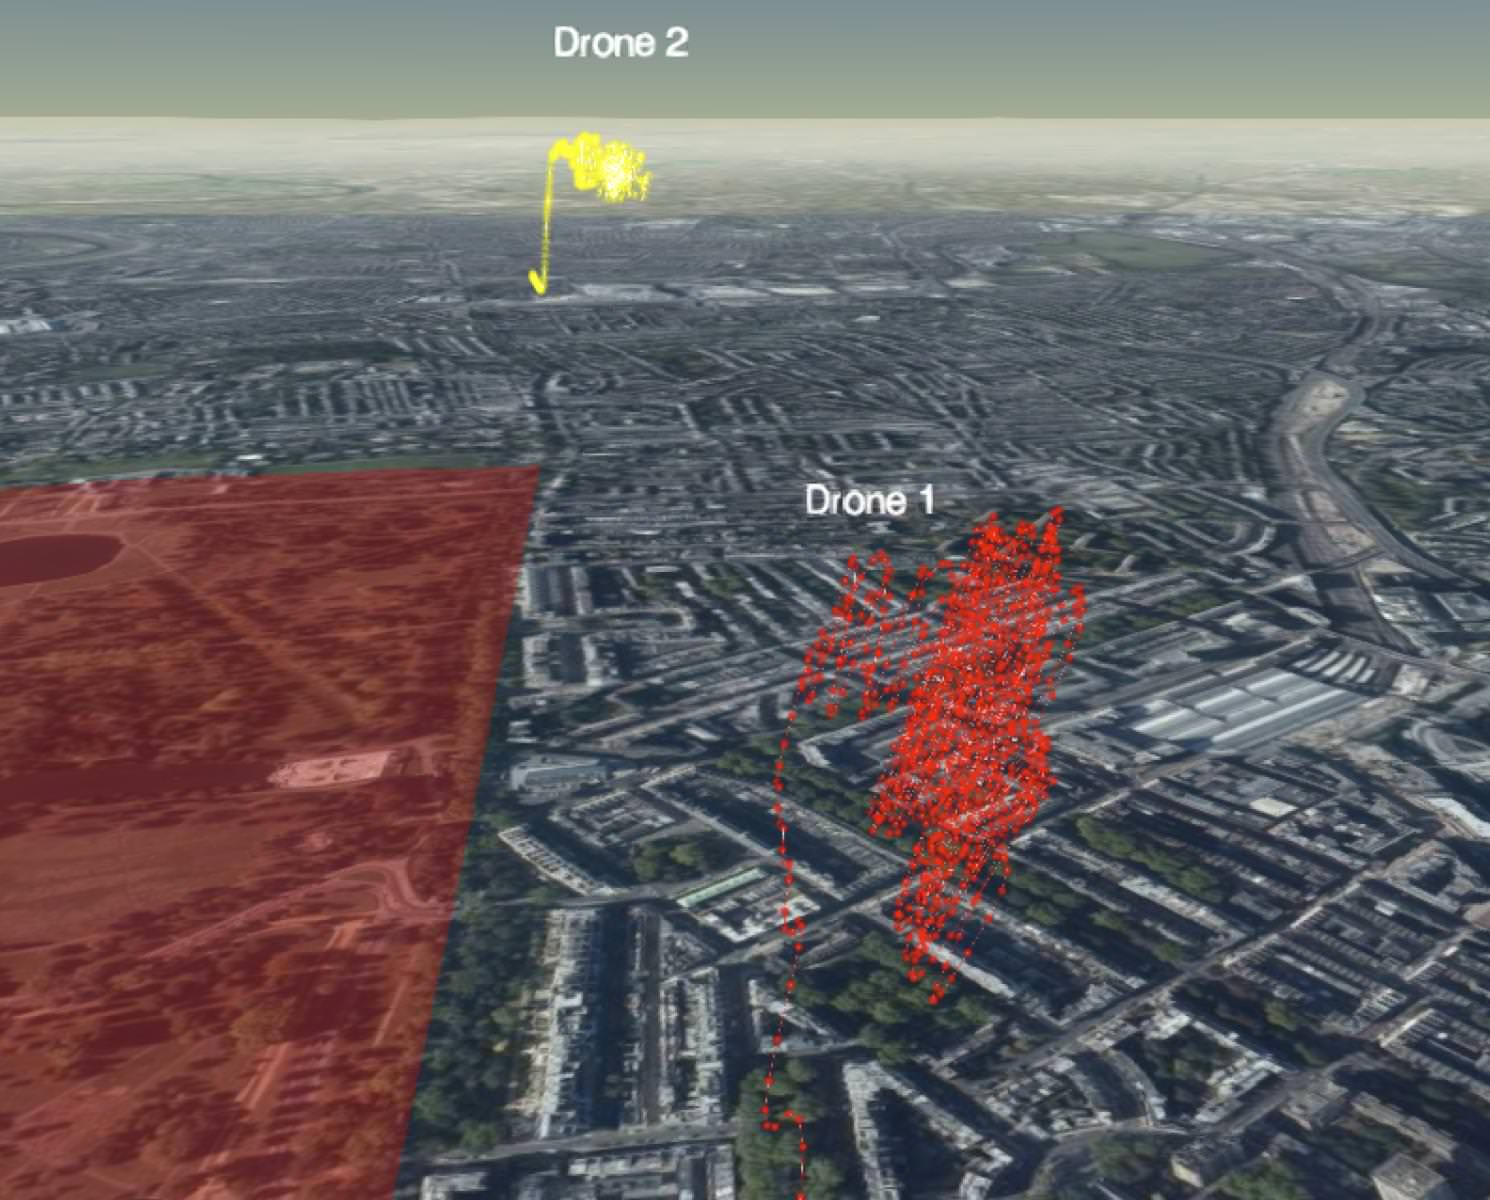
\includegraphics[width=\linewidth]{img/aatc_spaghett.jpg}
  \caption{Drone paths after increasing repulsion constant by 3 orders of magnitude.}
  \label{fig:aatc_spaghett}
\end{figure}

Effectively, an initial range of values (see Table \ref{tab:gen_alg}) is provided and the genetic algorithm cycles through all of these, letting these constants compete against each other to see which set of constants produces the simulation with the lowest cost. This cost is determined from a cost function that returns the remaining battery life of a drone if it reaches its destination, or a relatively huge number otherwise.
$$cost = \sum_{testcase} \sum_{drone}
    \begin{cases}
      batteryUsed & if \; drone \; reached \; destination    \\
      100000 & otherwise \\

   \end{cases}$$

\begin{table}[!hbpt]
\centering
\begin{tabular}{|l|l|l|l|l|}
\hline
Constant           & Min & Max & Step & Total \\ \hline
Attraction         & 0.8 & 1.1 & 0.1    & 3     \\ \hline
Repulsion          & 100 & 500 & 100  & 5     \\ \hline
Return             & 0.1 & 0.7 & 0.2  & 4     \\ \hline
Influence distance & 300 & 600 & 100  & 4     \\ \hline
\multicolumn{4}{|l|}{Population}      & 240   \\ \hline
\end{tabular}
\caption{Initial configuration of the genetic algorithm for AATC. \cite{Balaji2017}}
\label{tab:gen_alg}
\end{table}

\subsubsection{Conclusions}
In the end, the genetic algorithms only improved the simulations by about 2\%\cite{Balaji2017} which could mean that the original range of constants was already a good set to work with. However, there is still scope for even greater improvements if the genetic algorithm was to be run with a greater number of test scenarios, bigger range of values to cycle through, and generally larger simulations.

\subsection{Scheduling Algorithms}
In this section we look at a few well known CPU scheduling algorithms\cite{Bell2018}. Although CPU scheduling is not part of this project, being able to understand a few different approaches to the problem will give insight into how to schedule drones later on. However, there are two key difference between drone and CPU scheduling.\\

The first is that CPUs can time slice different tasks whereas once a drone is scheduled onto a task, it has to complete the whole task before being able to pick up a new one. Secondly, there are vastly more drones that could be running at a point in time compared to the number of cores in multi-core CPU, leading to far greater parallelism.

\subsubsection{First Come First Serve (FCFS)}
As the title says, this algorithm operates as a FIFO queue where tasks are scheduled in the same order that they arrive. Some might consider this the fairest form of scheduling, since it does not discriminate against any task, but simply prioritises the one that arrived soonest.

\subsubsection{Shortest Job First (SJF)}
This approach looks at the time each incoming task would take to complete, and puts the shortest task at the front of the schedule. While this means that small tasks get completed quickly, a constant stream of small tasks could mean that any heavier tasks never get scheduled or completed.

\subsubsection{Priority Scheduling}
Priority scheduling is a more general case of SJF, since each task is now given a priority - defined either internally or externally - and tasks with the highest priority are scheduled first. In SJF, the inverse of the estimated job time is used as the priority.

\subsubsection{Multi-Level Feedback Queue (MLFQ)}
MLFQ is an extension of an ordinary multi-level queue, where there are several queues of tasks to be completed and tasks are scheduled from non-empty queues in a round-robin fashion. A benefit of this approach is that each queue could be running different scheduling algorithms that better fits the priority of that queue.\\

\begin{figure}[!hbpt]
  \center
  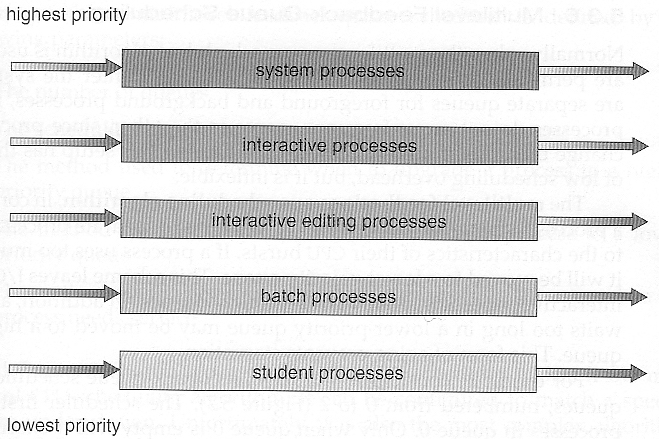
\includegraphics[width=0.6\linewidth]{img/mlqs.jpg}
  \caption{Multiple levels of queues, scheduled in a round-robin fashion. \cite{Bell2018}}
  \label{fig:mlqs}
\end{figure}

The ``feedback'' element of MLFQ allows tasks to be moved from one queue to another, depending on changes of circumstances. For example, if a queue has been left in a low priority queue for long enough, it may be moved to a higher priority queue - thus improving the chance that all incoming tasks get scheduled at some point in time.

\begin{figure}[!hbpt]
  \center
  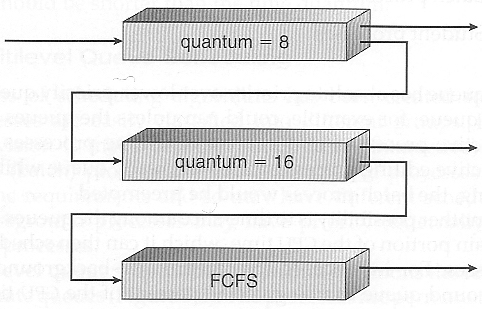
\includegraphics[width=0.6\linewidth]{img/mlfqs.jpg}
  \caption{Arrows indicate tasks can be moved up one queue to another. \cite{Bell2018}}
  \label{fig:mlfqs}
\end{figure}

\subsection{TODO: Time-Value of Data}

\subsubsection{Relation to Quality of Service}
\subsubsection{Relevance to Drones}


\newpage
\subsection{SpatialOS}
SpatialOS is a platform, created by \textit{Improbable}\cite{ImprobableWorldsLtd.2018a}, for running massive-scale simulated worlds. In their own words\cite{ImprobableWorldsLtd.2018b}:
\begin{displayquote}
SpatialOS is a cloud-based computational platform that lets you use many servers and engines to power a single world. The platform coordinates a swarm of micro-services called workers, which overlap and dynamically reorganize to power a huge, seamless world. The platform also lets you handle a huge number of concurrent players across different devices in one world.
\end{displayquote}

Although most commonly used for large distributed game worlds, SpatialOS has been used for simulating cities\cite{Narula2017}, the backbone of the Internet\cite{ImprobableWorldsLtd.2016} and a model of the brain\cite{ImprobableWorldsLtd.2018}. It is an ideal platform for simulating ``independent entities that have a location in space''\cite{ImprobableWorldsLtd.2018}.

\begin{figure}[!hbpt]
\centering
\begin{subfigure}{.5\textwidth}
  \centering
  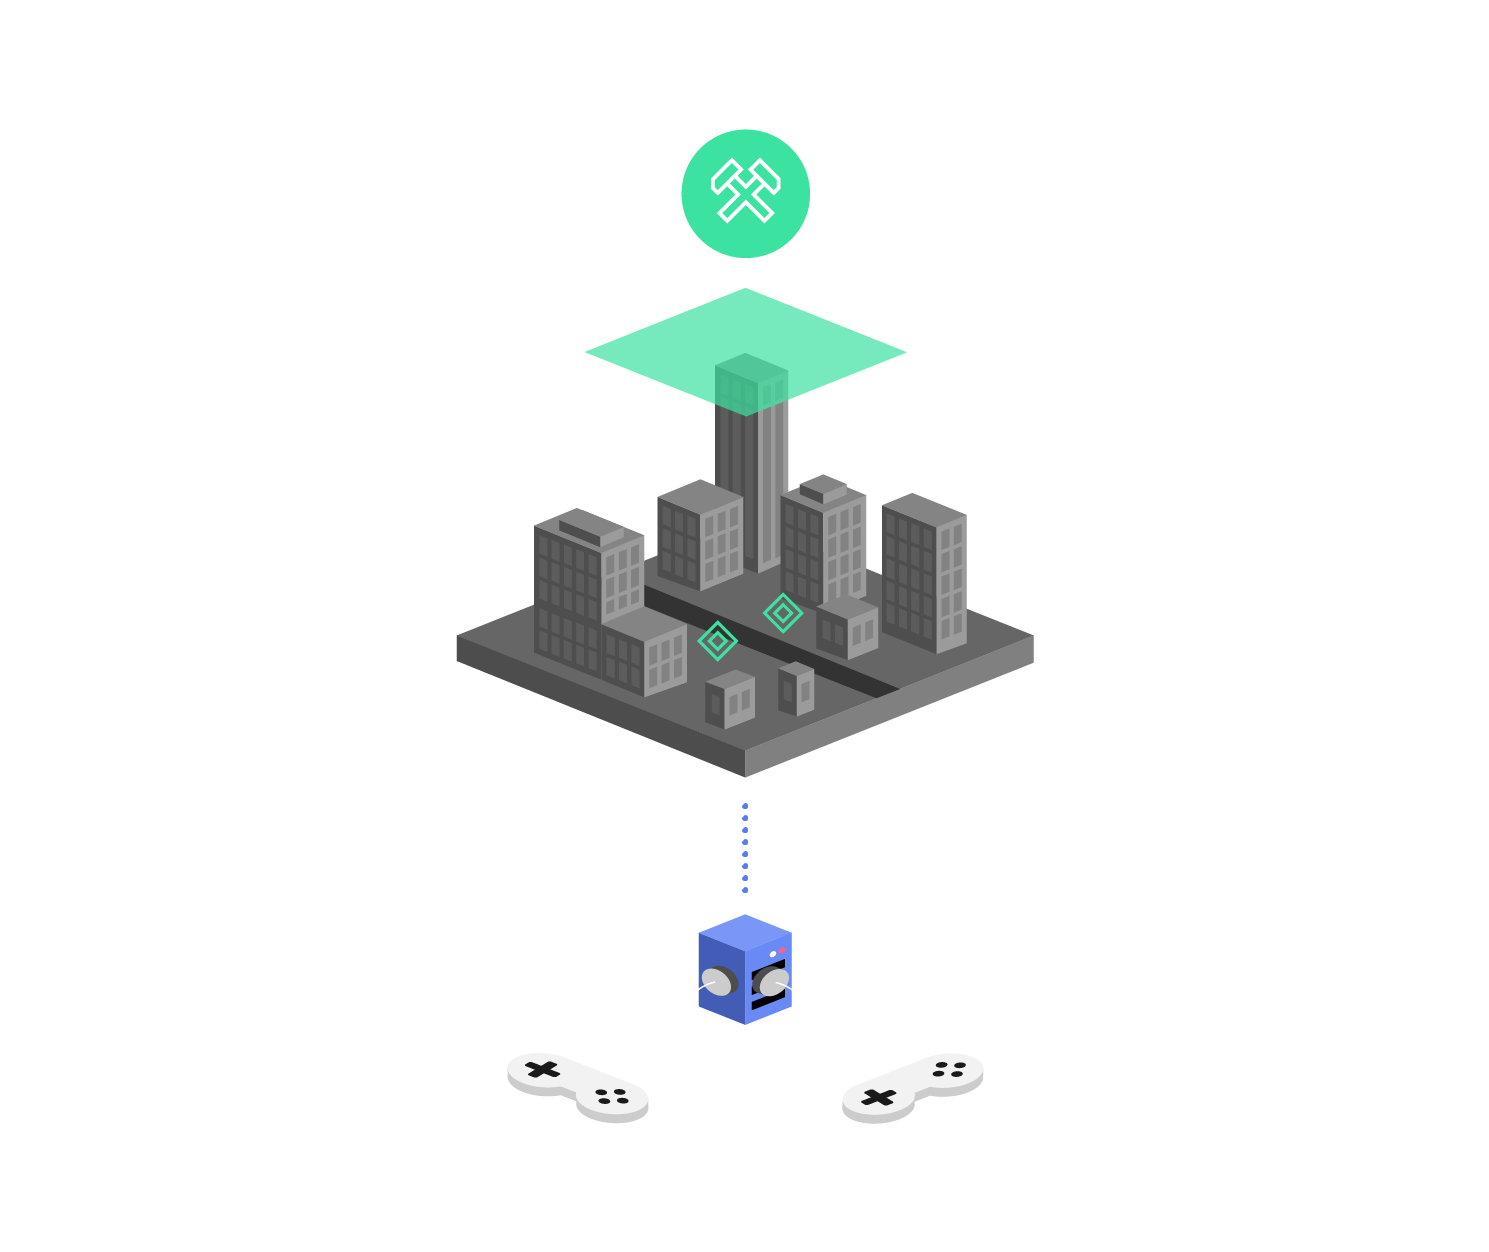
\includegraphics[width=\linewidth]{img/spatialos-diagram_current2.png}
  \caption{The current approach.}
  \label{fig:spatialos-diagram_current2}
\end{subfigure}%
\begin{subfigure}{.5\textwidth}
  \centering
  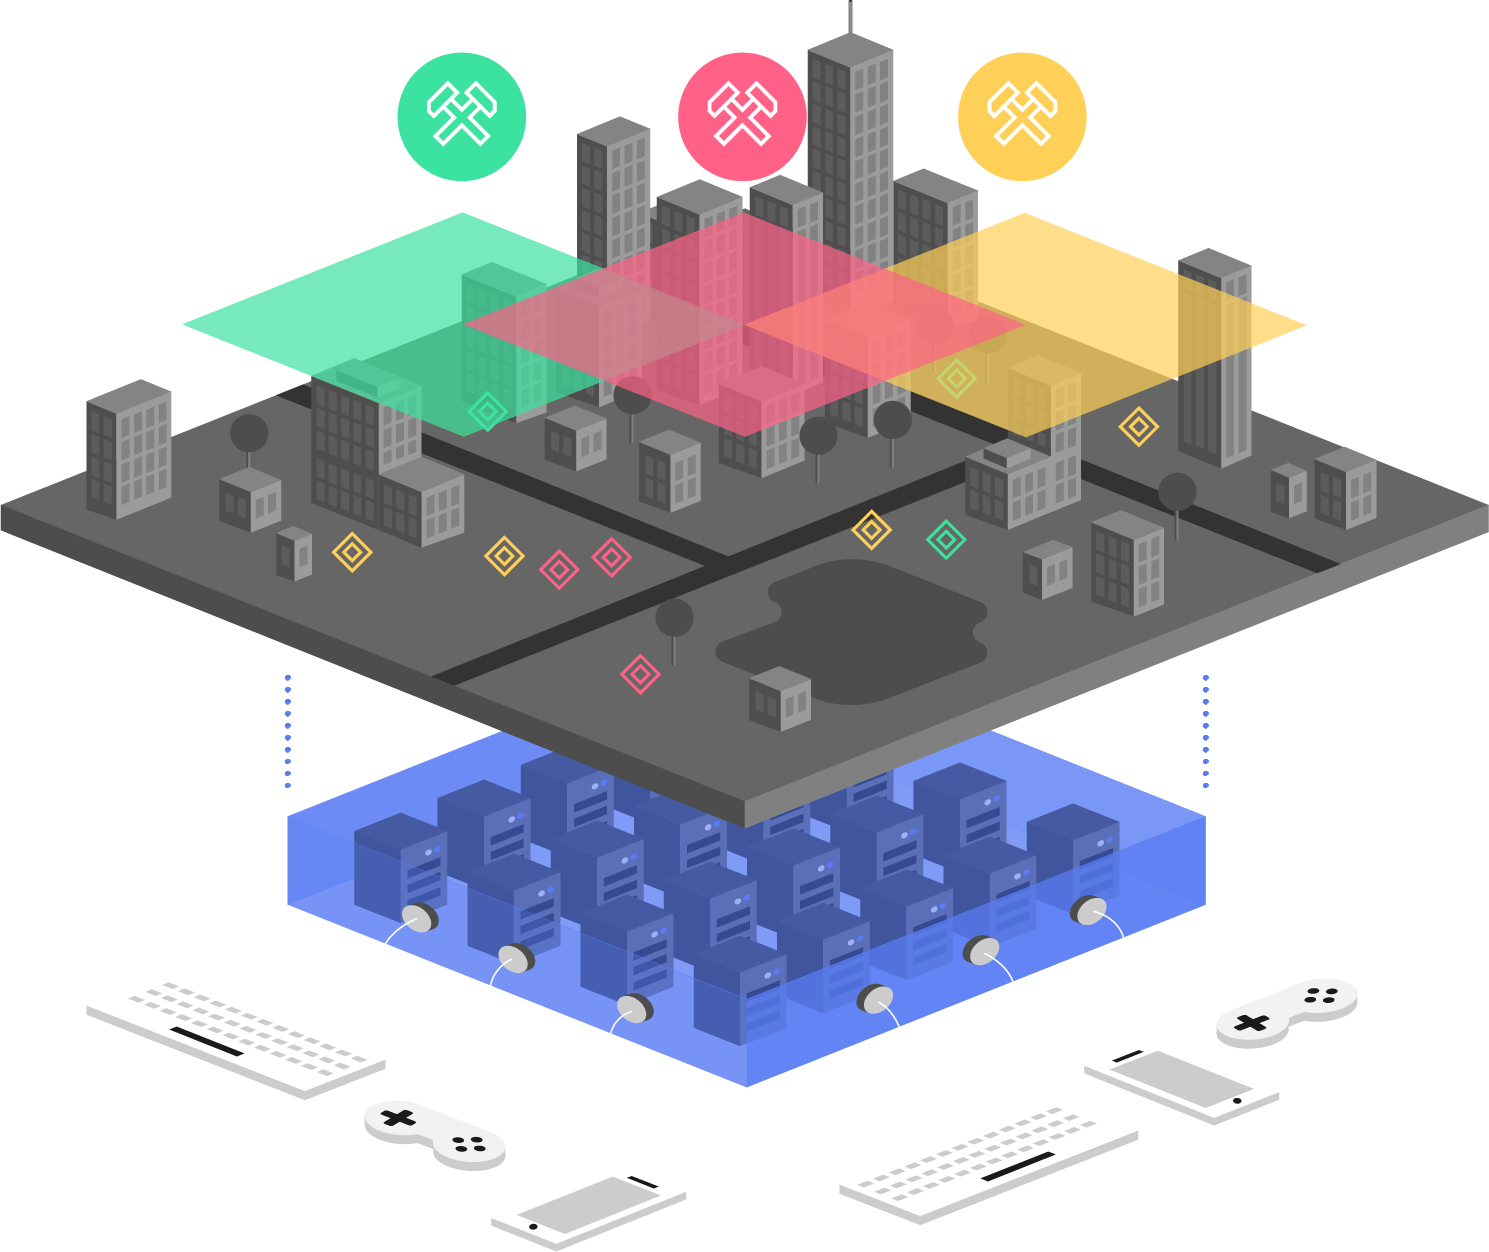
\includegraphics[width=\linewidth]{img/spatialos-diagram_solution2.png}
  \caption{How SpatialOS is different.}
  \label{fig:spatialos-diagram_solution2}
\end{subfigure}
\caption{Comparing approaches to multiplayer. \cite{ImprobableWorldsLtd.2018b}}
\label{fig:test}
\end{figure}

Anybody is able to sign up and use SpatialOS to build games using either the Unity3D or Unreal game engines. Alternatively, one can use the C\#, C++ and Java SDKs to create custom workers to be ran on SpatialOS deployments. \\

A benefit of SpatialOS's Unity and Unreal SDKs is that creating a sole game client, without manually writing network code, is almost enough to get multiplayer built-in to the game for ``free'', i.e. taken as granted.

\subsubsection{Unity SDK}
Of the two game engine integrations, the Unity SDK is arguably the most stable because it has been in development for far longer than the Unreal SDK, and it is not in beta. From prior industrial experience, the Unity integration is also easier to implement quick prototypes with and iterate on.

\subsubsection{Abstraction}
SpatialOS adopts an \textbf{Entity}-\textbf{Component}-\textbf{Worker} model.
\begin{itemize}
  \item \textbf{Entities} are anything in the world that have a position.
  \item \textbf{Components} define state and how other entities interact with them.
  \item \textbf{Workers} are micro-services that simulate components of entities in the world.
\end{itemize}

\subsubsection{Developer Tools}
There is extensive logging of performance metrics, which is a fantastic starting point for scaling up a simulation\cite{Brighting}. In addition to this, there is an active developer \textbf{Forum} - where SpatialOS developers and Improbable engineers meet to help other SDK users solve their problems\cite{ImprobableWorldsLtd.2018c}. \\

Naturally as the public SDKs have matured, so too have the public-facing developer tools. Currently, there is an \textbf{Inspector} to view the location of entities and the values that their components have at a given time, in either a local or deployed simulation.

\begin{figure}[!hbpt]
  \center
  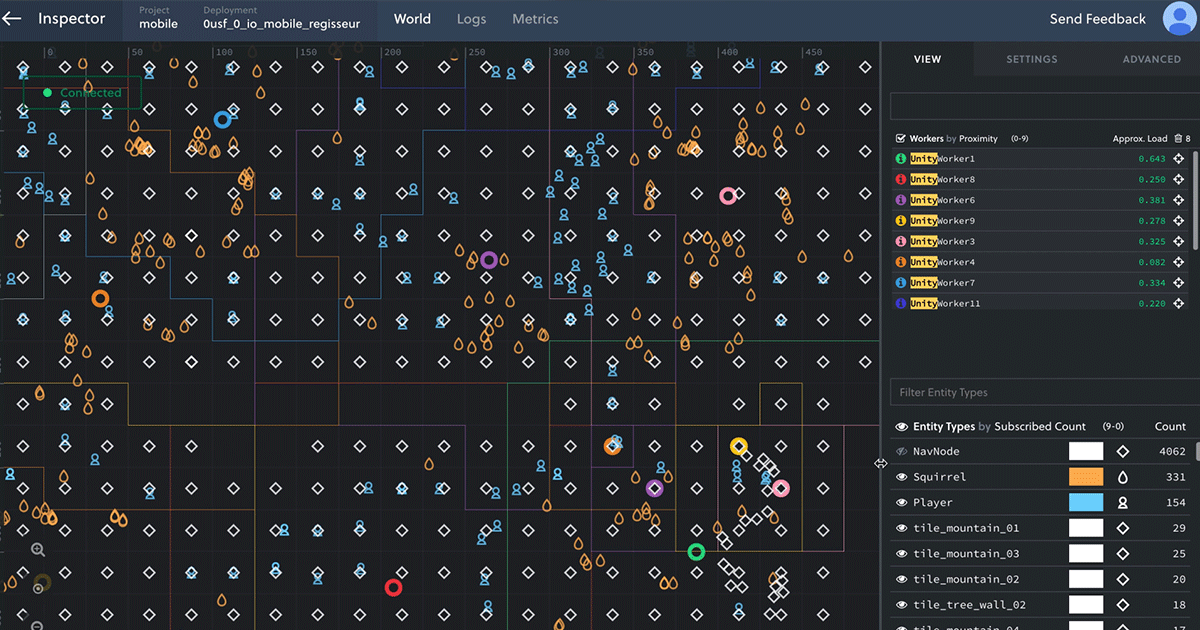
\includegraphics[width=\linewidth]{img/io_inspector.png}
  \caption{The Inspector demonstrating a deployment of the iOS Demo, \textit{Quest}. \cite{ImprobableWorldsLtd.2017}}
  \label{fig:bg_scalable_zones}
\end{figure}

\subsubsection{Layered Simulation}
By virtue of games having several dynamic systems all interlinking with each other, it is possible to create layered simulations on SpatialOS. This works well with the concept of Global, Reactive and Zonal layers that have been mentioned already in Sections 2.4, 2.5 and 2.6. Furthermore, as SpatialOS is distributed by nature, it is the ideal platform to create and execute massive layered, distributed simulations.


%**********************************************%
\newpage
\section{TODO: Drone-Controller Architecture}
blabla

%**********************************************%
\newpage
\section{TODO: Order Generation}
blabla

%**********************************************%
\newpage
\section{TODO: London Snapshot Generation}
blabla

%**********************************************%
\newpage
\section{TODO: Scheduling Deliveries}
blabla

%**********************************************%
\newpage
\section{TODO: Prioritising Economic Value}
Thus far, we have shown that whilst there is great scope to utilise drones for delivery of physical goods, the existing implementation of AATC only touches upon the routing aspect - how to get from point A to point B. Even in all the test cases, the drones' start and end points were hand-picked by the developers\cite{Balaji2017} to give an insight into how AATC would operate in a variety of scenarios. \\

To gain greater understanding of how drones can positively impact industries, simulations need to be performed which take into account the financial aspect of their use case. For example when it comes to drone delivery networks, we want to ensure that the drones not only reach their destination quickly, but that they also get scheduled and utilised in the appropriate manner to maximise the profitability of the network.

\subsection{Time Value Functions}
In order to consider how to maximise profitability, we introduce the concept of a Time Value Function (TVF). Rather than deal with the fixed pricing model of delivery fees as we see in the current day, we propose a new mechanism where the cost of the delivery is a function of the time taken to do said delivery. For example, a user may pay £5 for a delivery within 30 minutes but might be charged nothing if it takes longer than one hour.\\

%**********************************************%
\newpage
\section{TODO: Large Scale Simulation of London}
blabla

%**********************************************%
\newpage
\section{TODO: Evaluation}
blabla

%**********************************************%
\newpage
\section{TODO: Conclusion \& Future Work}
blabla

%**********************************************%
\newpage
\addcontentsline{toc}{section}{References}

\printbibliography

% \newpage
% \begin{appendices}
% \end{appendices}

\end{document}
